%!TEX root = fastZKP.tex

\section{Implementations and Evaluations}\label{sec:eval}

\textbf{Settings.} We use C++ to implement our zero knowledge protocol including circuit generator, zk-GKR and zk-VPD. Besides, we write a new large integer class named u512 combined with GMP\cite{GNU} for field arithmetic. For the binary pairing, we use the ate-pairing\cite{ate-pairing} library on a 254-bit elliptic curve.\\
We run all of the experiments on an Amazon EC2 m4.2xlarge machine having 32GB of RAM and an Intel Xeon E5-2686v4 CPU with eight 2.3GHz virtual cores. Our implementations are not parallelized and only use a single CPU core.\\

\paragraph{Key generation with lookup tables.}

\paragraph{More gate types with no overhead.}

\subsection{Improvements on GKR protocols}\label{subsec:expGKR}
\paragraph{Methodology.} In the section, we would compare our GKR system with previous various GKR system on several types of the circuit listed below to verify the optimal prove time in practice. In order to obtain the unbiased result, we reimplement all of these GKR systems in C++ with the same C++ library. 
\begin{itemize}
	\item Regular circuit is the circuit that has a very good structure. More general, there are two map funtions that take the arbitrary gate as the input and output the corresponding two input gates of this gate. The prove time could be improved to linear of the circiut size\cite{JT_Thesis}.
	\item Single-instruction multi-data circuit means the circuit $C$ could be divided into several parallel copies of sub circuit $C'$, whose maximum number of gates at any layer is $S'$. Suppose the total number of copies is $B$, then the prove time could be $\mathcal{O}(BC'\log S')$ proposed by Zhang \etal \cite{zhang2017vsql}, then improved to $\mathcal{O}(BC' + C'\log S')$ by Wahby \etal \cite{wahby2017full}.   
	\item Multi-instruction multi-data circuit is similar to the above circuit but its parallel copies are not the same. The prove time of this circuit maintains $\mathcal{O}(BC'\log S')$.
	\item Generic circuit is the general layered arithmetic circuit, which is equivalent to the Turing machine. The previous best prove time of generic cuicuit is $\mathcal{C\log C}$, where $C$ is the size of the circuit\cite{CMT}.
\end{itemize}
\paragraph{Benchmarks.} We evaluate all of these systems on several benchmarks below. Considering some of these systems' efficiency only hold on suitable circuits, we choose corresponding functions subject to these properties. 
 \begin{itemize}
	\item
	\textbf{Matrix multiplication} means $\mathbb{P}$ proves to $\mathbb{V}$ that it knows two matrics whose product equals the public input. It is a basic function whose corresponding arithmetic cuicuit is regular and the depth is very small. We evaluate this function for matric of different sizes from 16x16 to 128x128. 
	\item
	\textbf{Image scaling} forces $\mathbb{P}$ to prove to $\mathbb{V}$ a low-definition image is a scaled version of a high-definition image. And we use a standard and classic image transformation method named Lanczos resampling\cite{Lanczos} to extend the picture. It uses the convolution of input image and windowed kernel function to produce the output pixels. And we use convolutional kernel function:
	\begin{equation}
	k(x)=\left\{
	\begin{aligned}
	&sinc(x)/sinc(ax), &\text{if} -a < x < a\\
	&0, &\text{otherwise}\\
	\end{aligned}
	\right.
	\end{equation}
	where $a$ is the parameter and $sinc(x) = sin(x)/x$. This function is data parallel where each sub-AC computes the same function to generate one pixel of the output image. We evaluate 16x scaling function on various sizes of pixels from 112x112 to 1072x1072.
	\item
	\textbf{Image scaling of different parameters} is very similar to the previous scaling. The only difference is that the parameter of the kernal function changes with window moves.
	So sub-ACs are still parallel but do not compute the same function. We evaluate the function with the same size of image scaling.
	\item
	\textbf{Random circuit} is an arithmatic circuit with depth three and constant gates for every layer. And we randomly sample the type of each gate, input value and the connection between adjacent circuit layers. We evaluate the random circuits of varying numbers of gates per layer from $2^{10}$ to $2^{20}$.
\end{itemize}
\begin{table*}[t!]
\centering
\begin{tabular}{|c|c|c|c|c|c|}
\hline
\multirow{3}{*}{\shortstack{Matrix\\ multiplication}} &Matrix size & 4x4 & 16x16 & 64x64 & 256x256\\ 
\cline{2-6}
{} & \cite{JT_Thesis} & 0.0003s & 0.0065s & 0.3923s & 28.9632s\\
\cline{2-6}
{} & Ours & 0.0004s & 0.0158s & 0.8663s & 55.1185s\\
\hline
\multirow{3}{*}{Image scaling} & \#pixels & 112x112 & 176x176 &560x560 & 1072x1072\\ 
\cline{2-6}
{} & \cite{wahby2017full} & 0.4848s & 0.8341s & 7.8867s & 30.7184s\\
\cline{2-6}
{} & Ours & 1.0865s & 4.1596s & 67.572s & 264.3290s\\
\hline
\multirow{3}{*}{\shortstack{Image scaling with\\ different parameters}} & \#pixels & 112x112 & 176x176 &560x560 & 1072x1072\\
\cline{2-6}
{} & \cite{zhang2017vsql} & 3 & 4 & 5 & 6\\
\cline{2-6}
{} & Ours & 3 & 4 & 5 & 6\\
\hline
\multirow{3}{*}{Random circuit} & \#gates per layer& $2^8$ & $2^{12}$ & $2^{16}$ & $2^{20}$\\ 
\cline{2-6}
{} & \cite{CMT} & 3 & 4 & 5 & 6\\
\cline{2-6}
{} & Ours & 3 & 4 & 5 & 6\\
\hline
\end{tabular}
\caption{\label{GKRCom}Comparison of the performance of \name{} versus various previous GKR systems.}
\end{table*}
\paragraph{Results.} As all of these systems implement the same protocol, proof size and verification time are exactly the same. Therefore, we only need to focus on the prove time of them. Experimental results are shown in Table \ref{GKRCom}. In conclusion, our protocol is comparable with previous protocols for regular circuit and data parallel circuit while much faster for multi-instruction multi-data circuit and random circuit. To be specific, for matrix multiplication, when the matrix size is 128x128, our protocol is about a litter slower than Thaler's protocol, that is because the constant coefficient of our protocol is larger. For image scaling, when the size of pixels are 112x112, our protocol is also a bit slower than Wahby's protocol, the same reason remains since the number of sub copies circuits are large. For image scaling with different parameters, when the number of pixels are 112x112, our protocol is 5x speed up since our algorithm is linear. 
For random circuit, when the number of gates per layer are $2^{20}$, our protocol is at least 10x speed up and this gap must be larger with circuit size grows.  
\subsection{Comparing to Other ZKP Schemes}\label{subsec:expZKP}
\textbf{Baselines.} In this section, we compare \name{} with previous state-of-the-art zero-knowledge argument systems with similar properties including Hyrax\cite{hyrax}, Ligero\cite{ligero}, Bulletproofs\cite{bulletproofs}, libSTARK\cite{libstark} and libSNARK\cite{libsnark}.
\begin{itemize}
\item
\textbf{Hyrax} is a zero-knowledge argument with quasi linear prove time, sublinear verification time, low communication complexity and no trusted setup. The implementation of their system is open source. Hence, we just run Hyrax under the same setting of our system.
\item
\textbf{Bulletproofs} is a zero knowledge argument with logarithmic prove time for range query. Since hyrax has implemented this system and released the code, we use the hyrax's implementation directly.
\item
\textbf{Ligero:} we report on the authors' C++ implementation.
\item
\textbf{libSTARK:} we report on the author's C++ implementation.
\item
\textbf{libSNARK:} we download their open source library and run their system on the same environment.
\end{itemize}
\paragraph{Benchmarks.} We evaluate \name{}, Hyrax, Bulletproofs, Ligero, libSNARK and libSTARK on matrix multiplication, image scaling and Merkle Tree\cite{merkletree}. Considering various properties of different systems and some constrains on implementation(\ie we do not have the sourse code of some systems), for each benchmark, we only evaluate the systems that is senseful and suitable for this benchmark.
\begin{itemize}
	\item
	\textbf{Merkle tree} means $\mathbb{P}$ proves to $\mathbb{V}$ it knows the value of the leaves of a Merkle tree\cite{merkletree} that computes the public root's value\cite{blum1994checking}. Same as the previous work, we use SHA-256 for the hash function. Besides, each sub-computation is one instance of the hash function which makes it data parallel. Therefore, if the Merkle tree has $M$ leaves, then we need $2M - 1$ sub-computations. We evaluate this function of varying number of leaves from 16 to 256.
\end{itemize}
\paragraph{Methodology.} For each benchmarks, we construct the corresponding arithmetic circuits of different sizes. Then we feed the circuit as the input into these zero knowledge systems. These systems would generate the proof and verify the proof itself. We measure the runtime using standard system clock.\\
\begin{figure}[htbp]
%\centering
\subfigure[Proof size: 64x64 matrix multiplication]{
%\begin{minipage}[t]{0.25\linewidth}
\centering
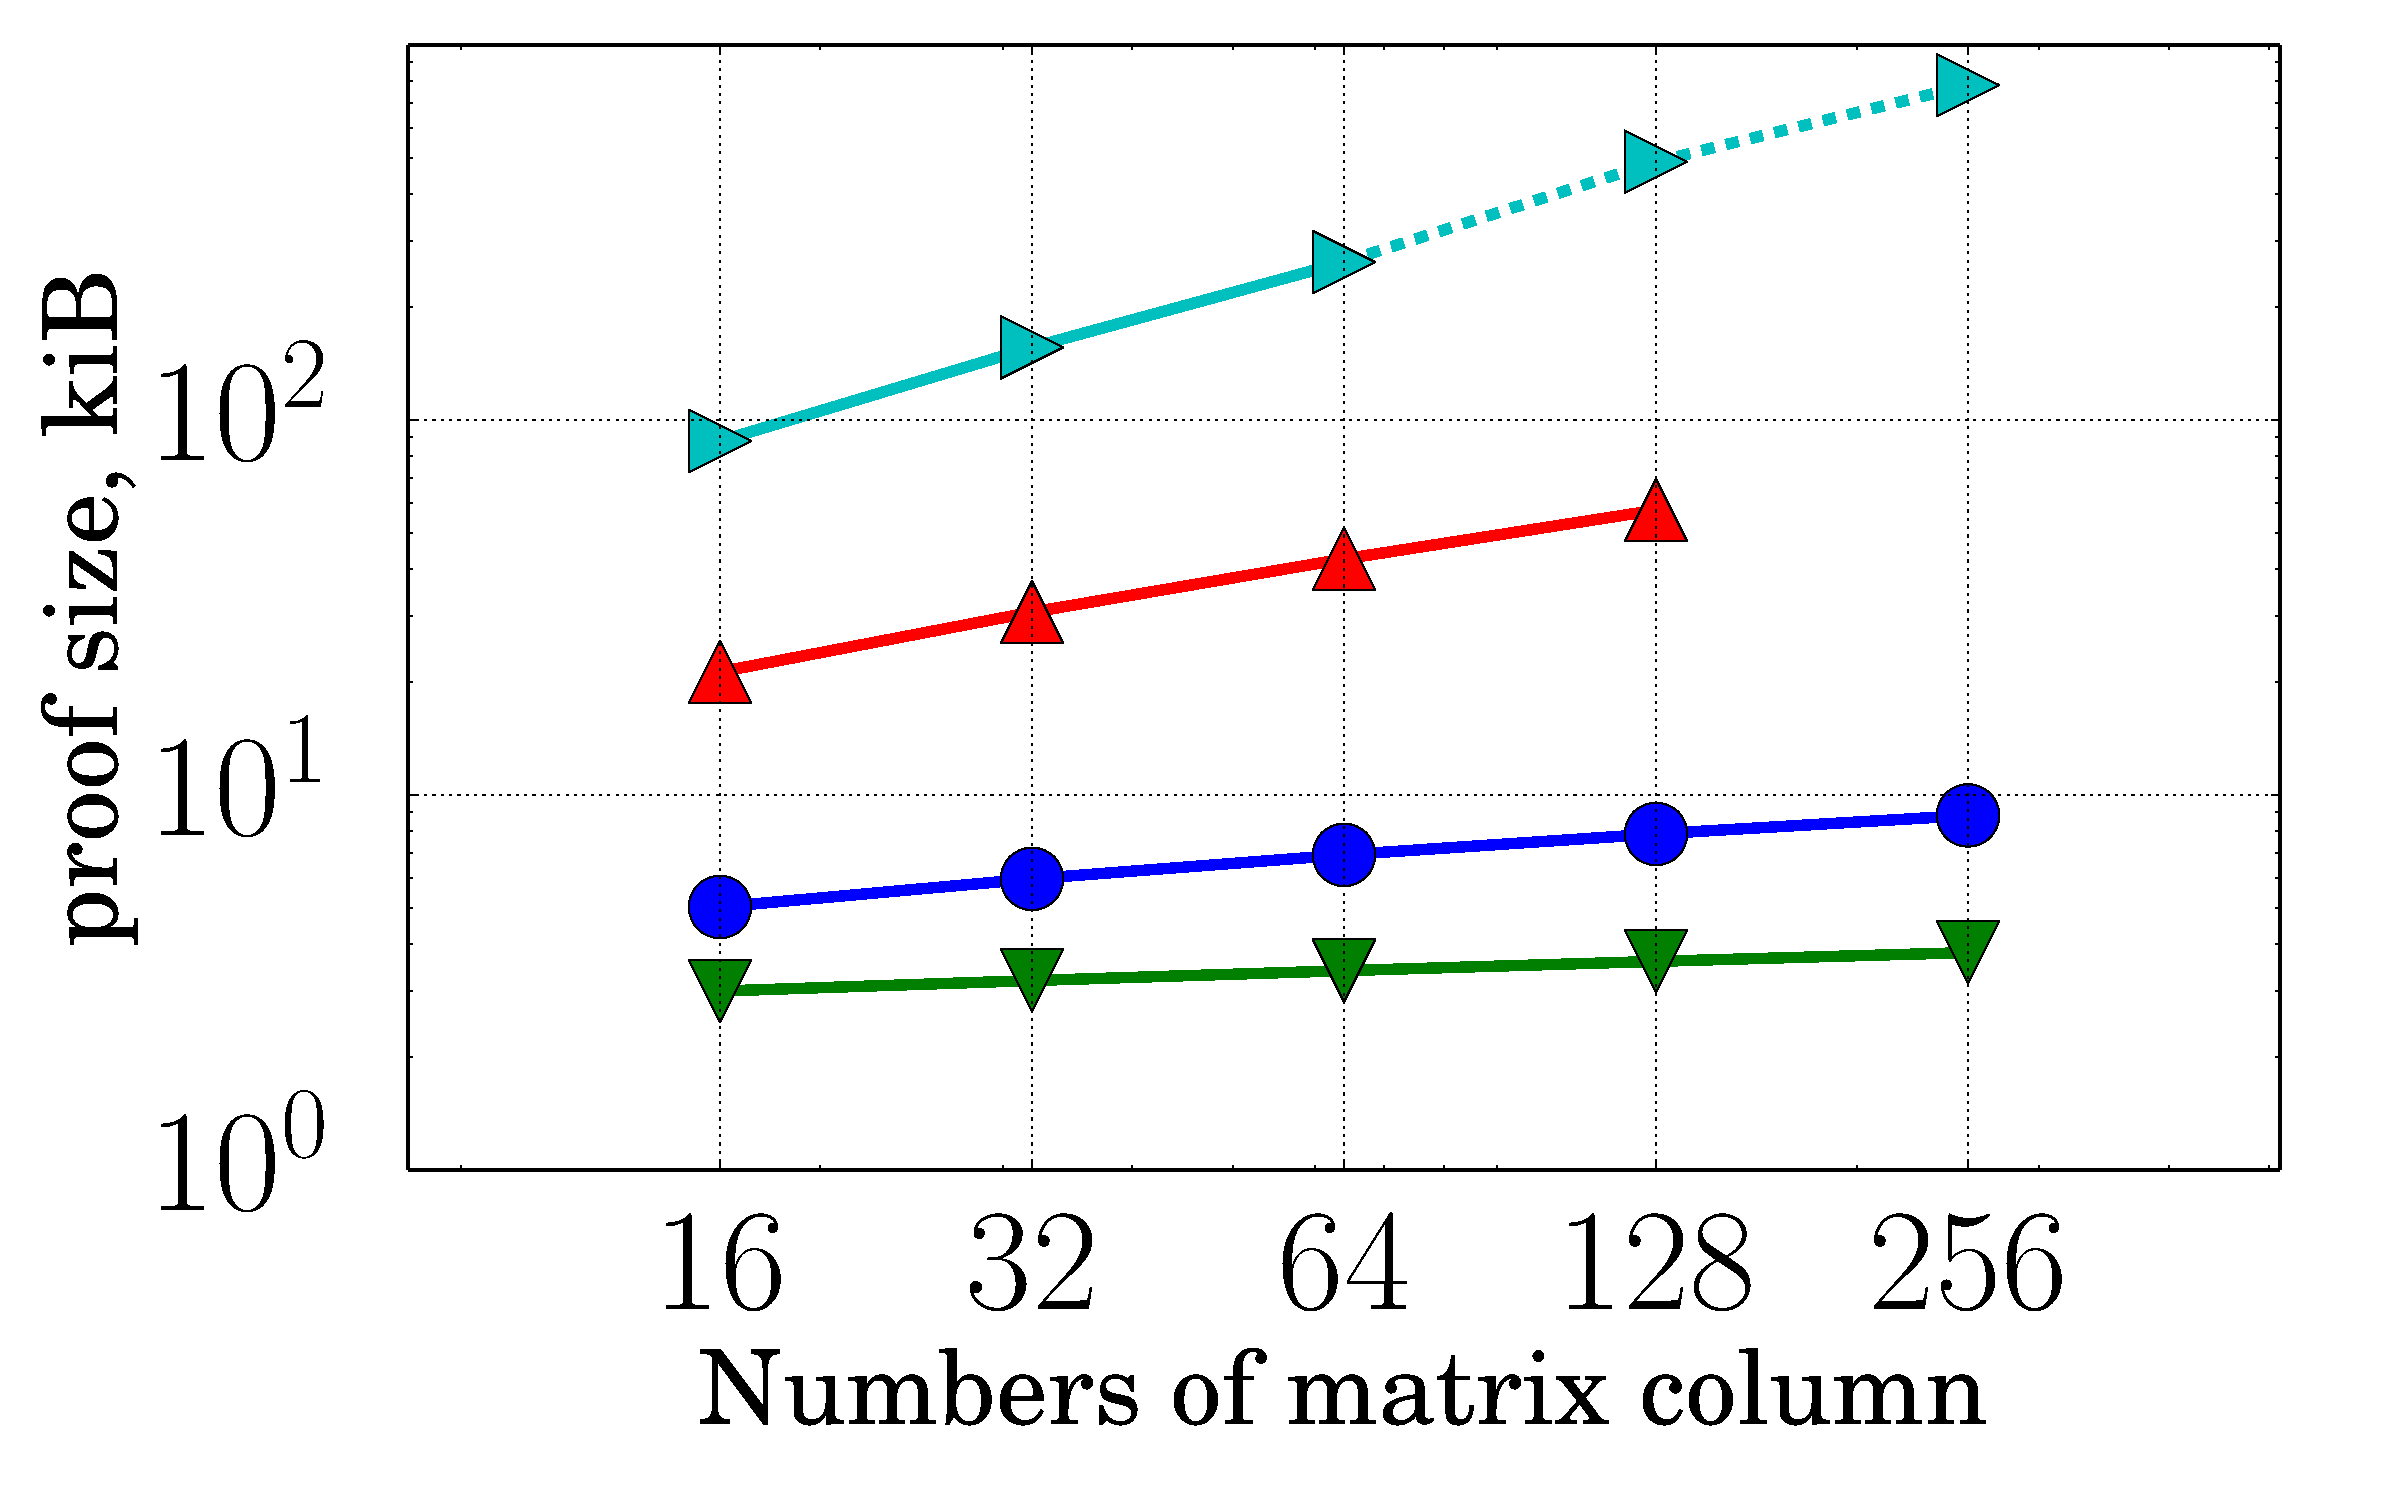
\includegraphics[width=2.1in]{fig1.pdf}
%\caption{fig1}
%\end{minipage}%
}%
%\hspace{0.05in}
\subfigure[Proof size: 16x Lanczos scaling]{
%\begin{minipage}[t]{0.25\linewidth}
%\centering
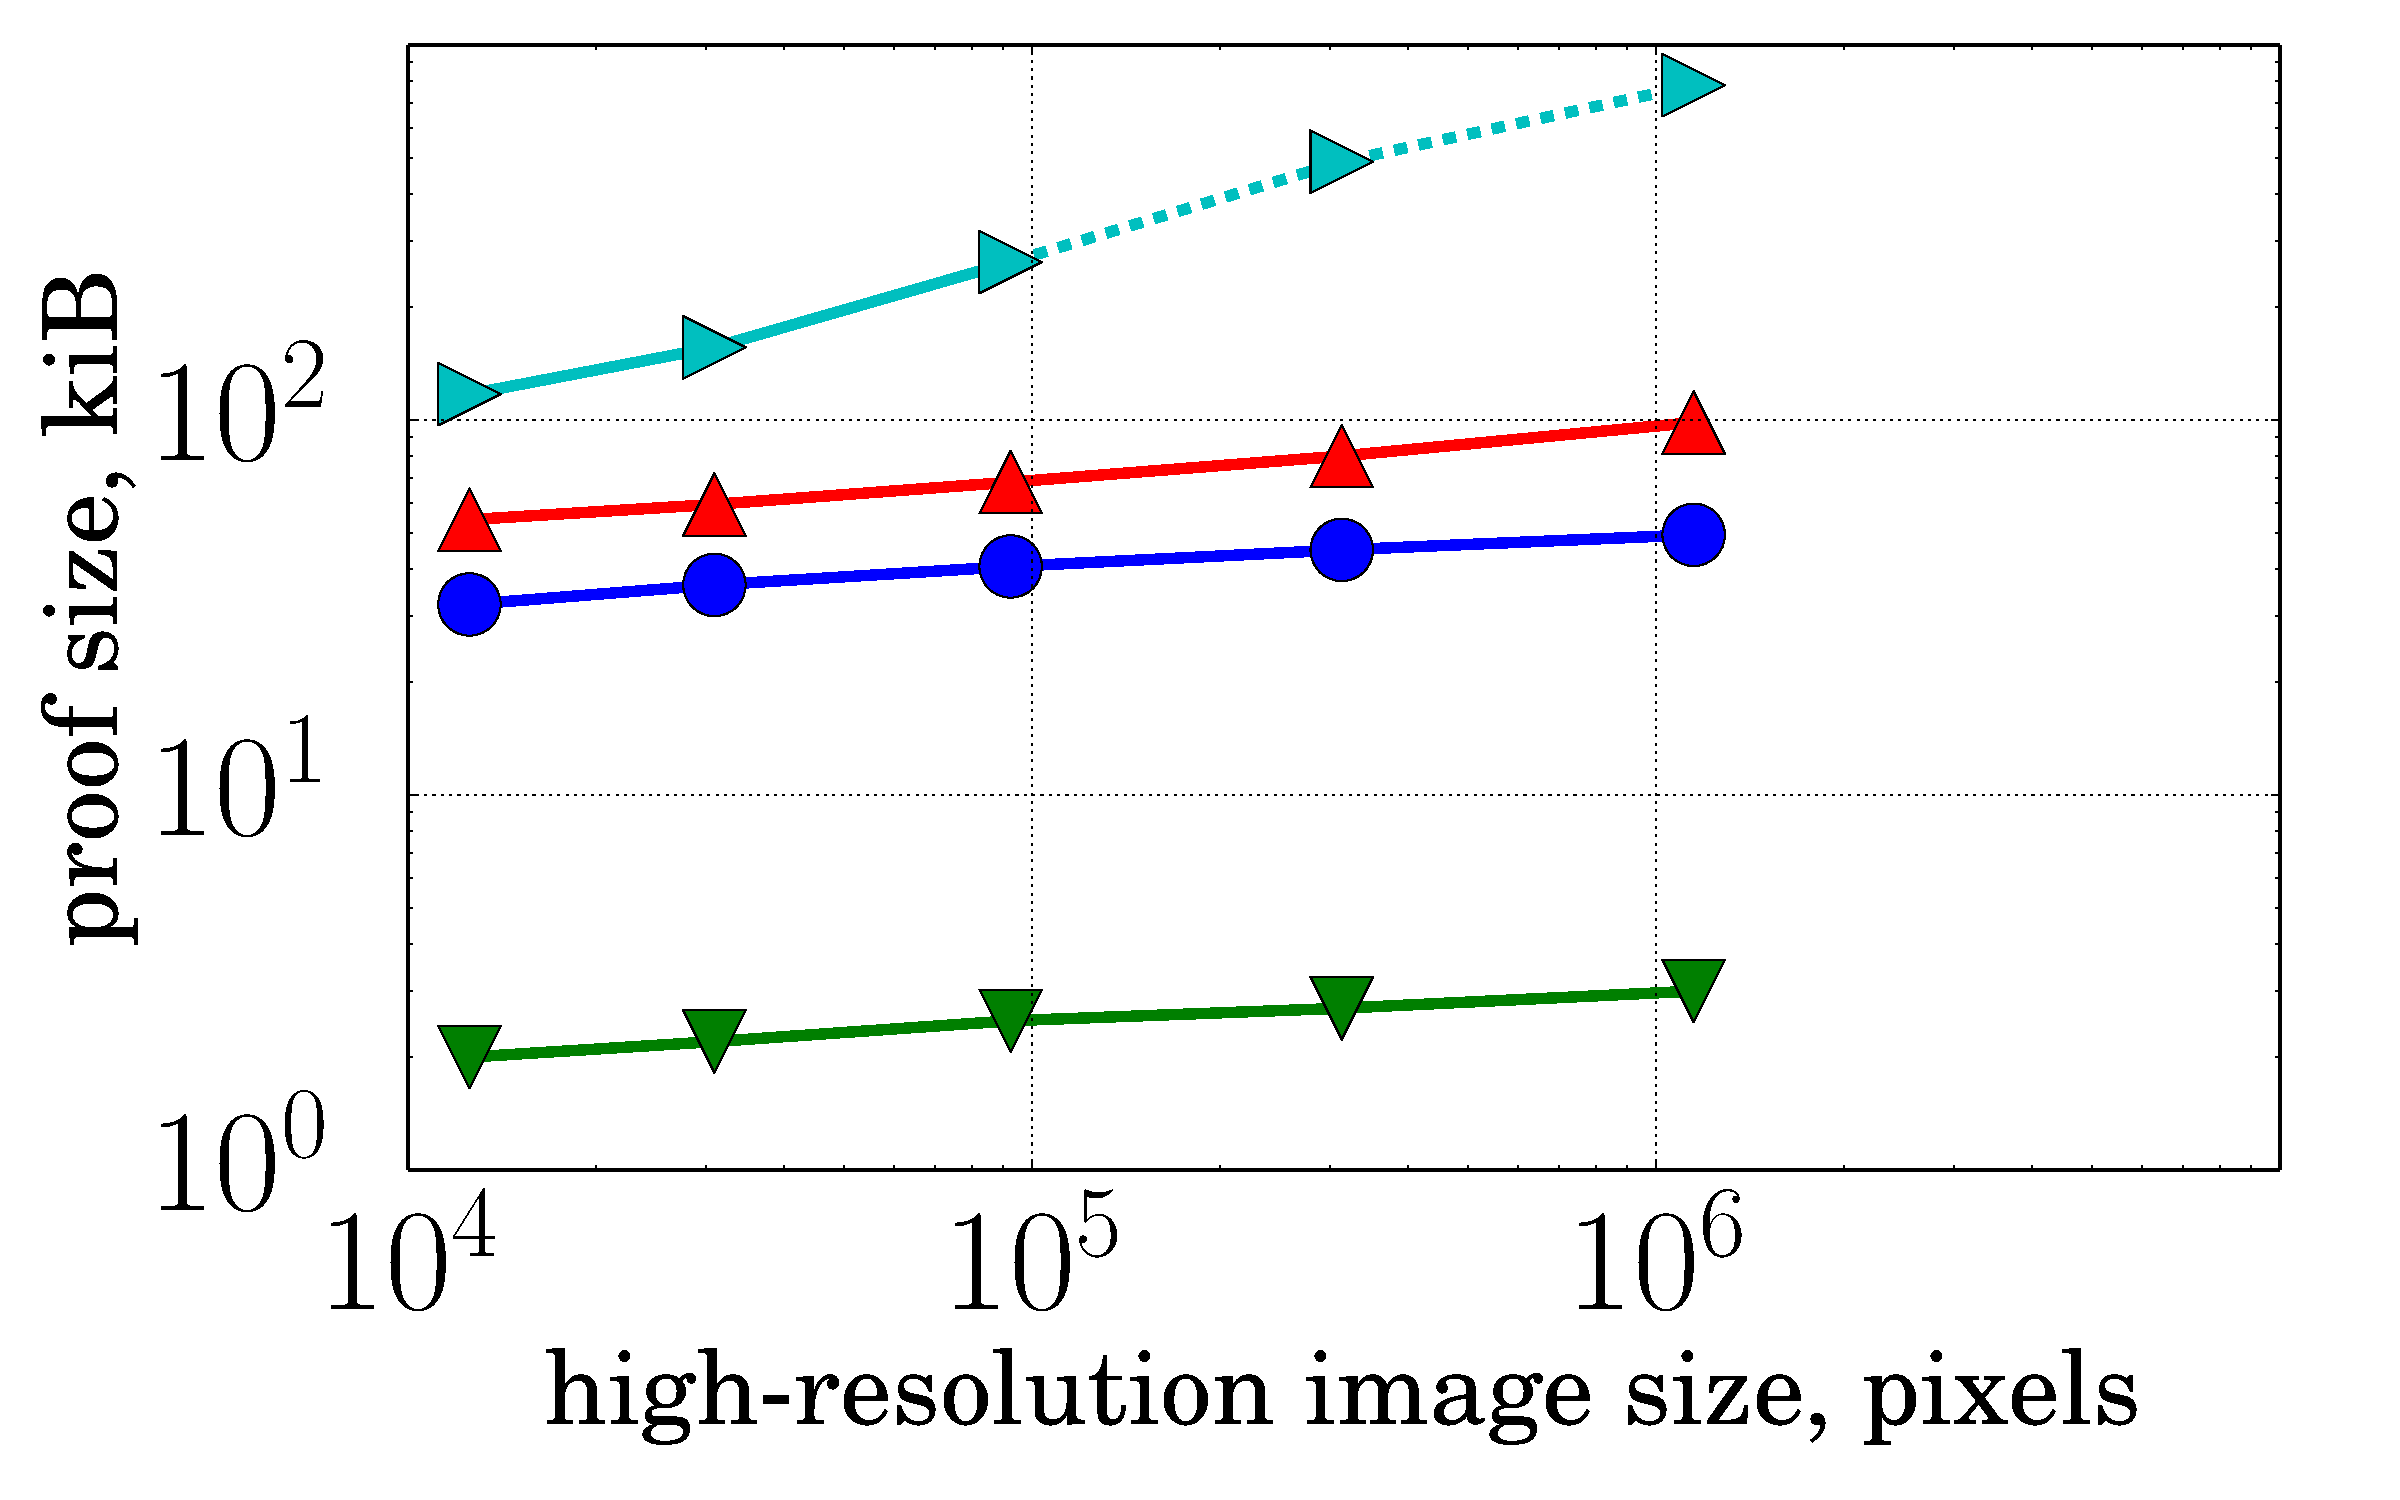
\includegraphics[width=2.1in]{fig2.pdf}
%\caption{fig2}
%\end{minipage}%
}%
%\hspace{0.05in}
\subfigure[Proof size: SHA-256 Merkle tree]{
%\begin{minipage}[t]{0.25\linewidth}
%\centering
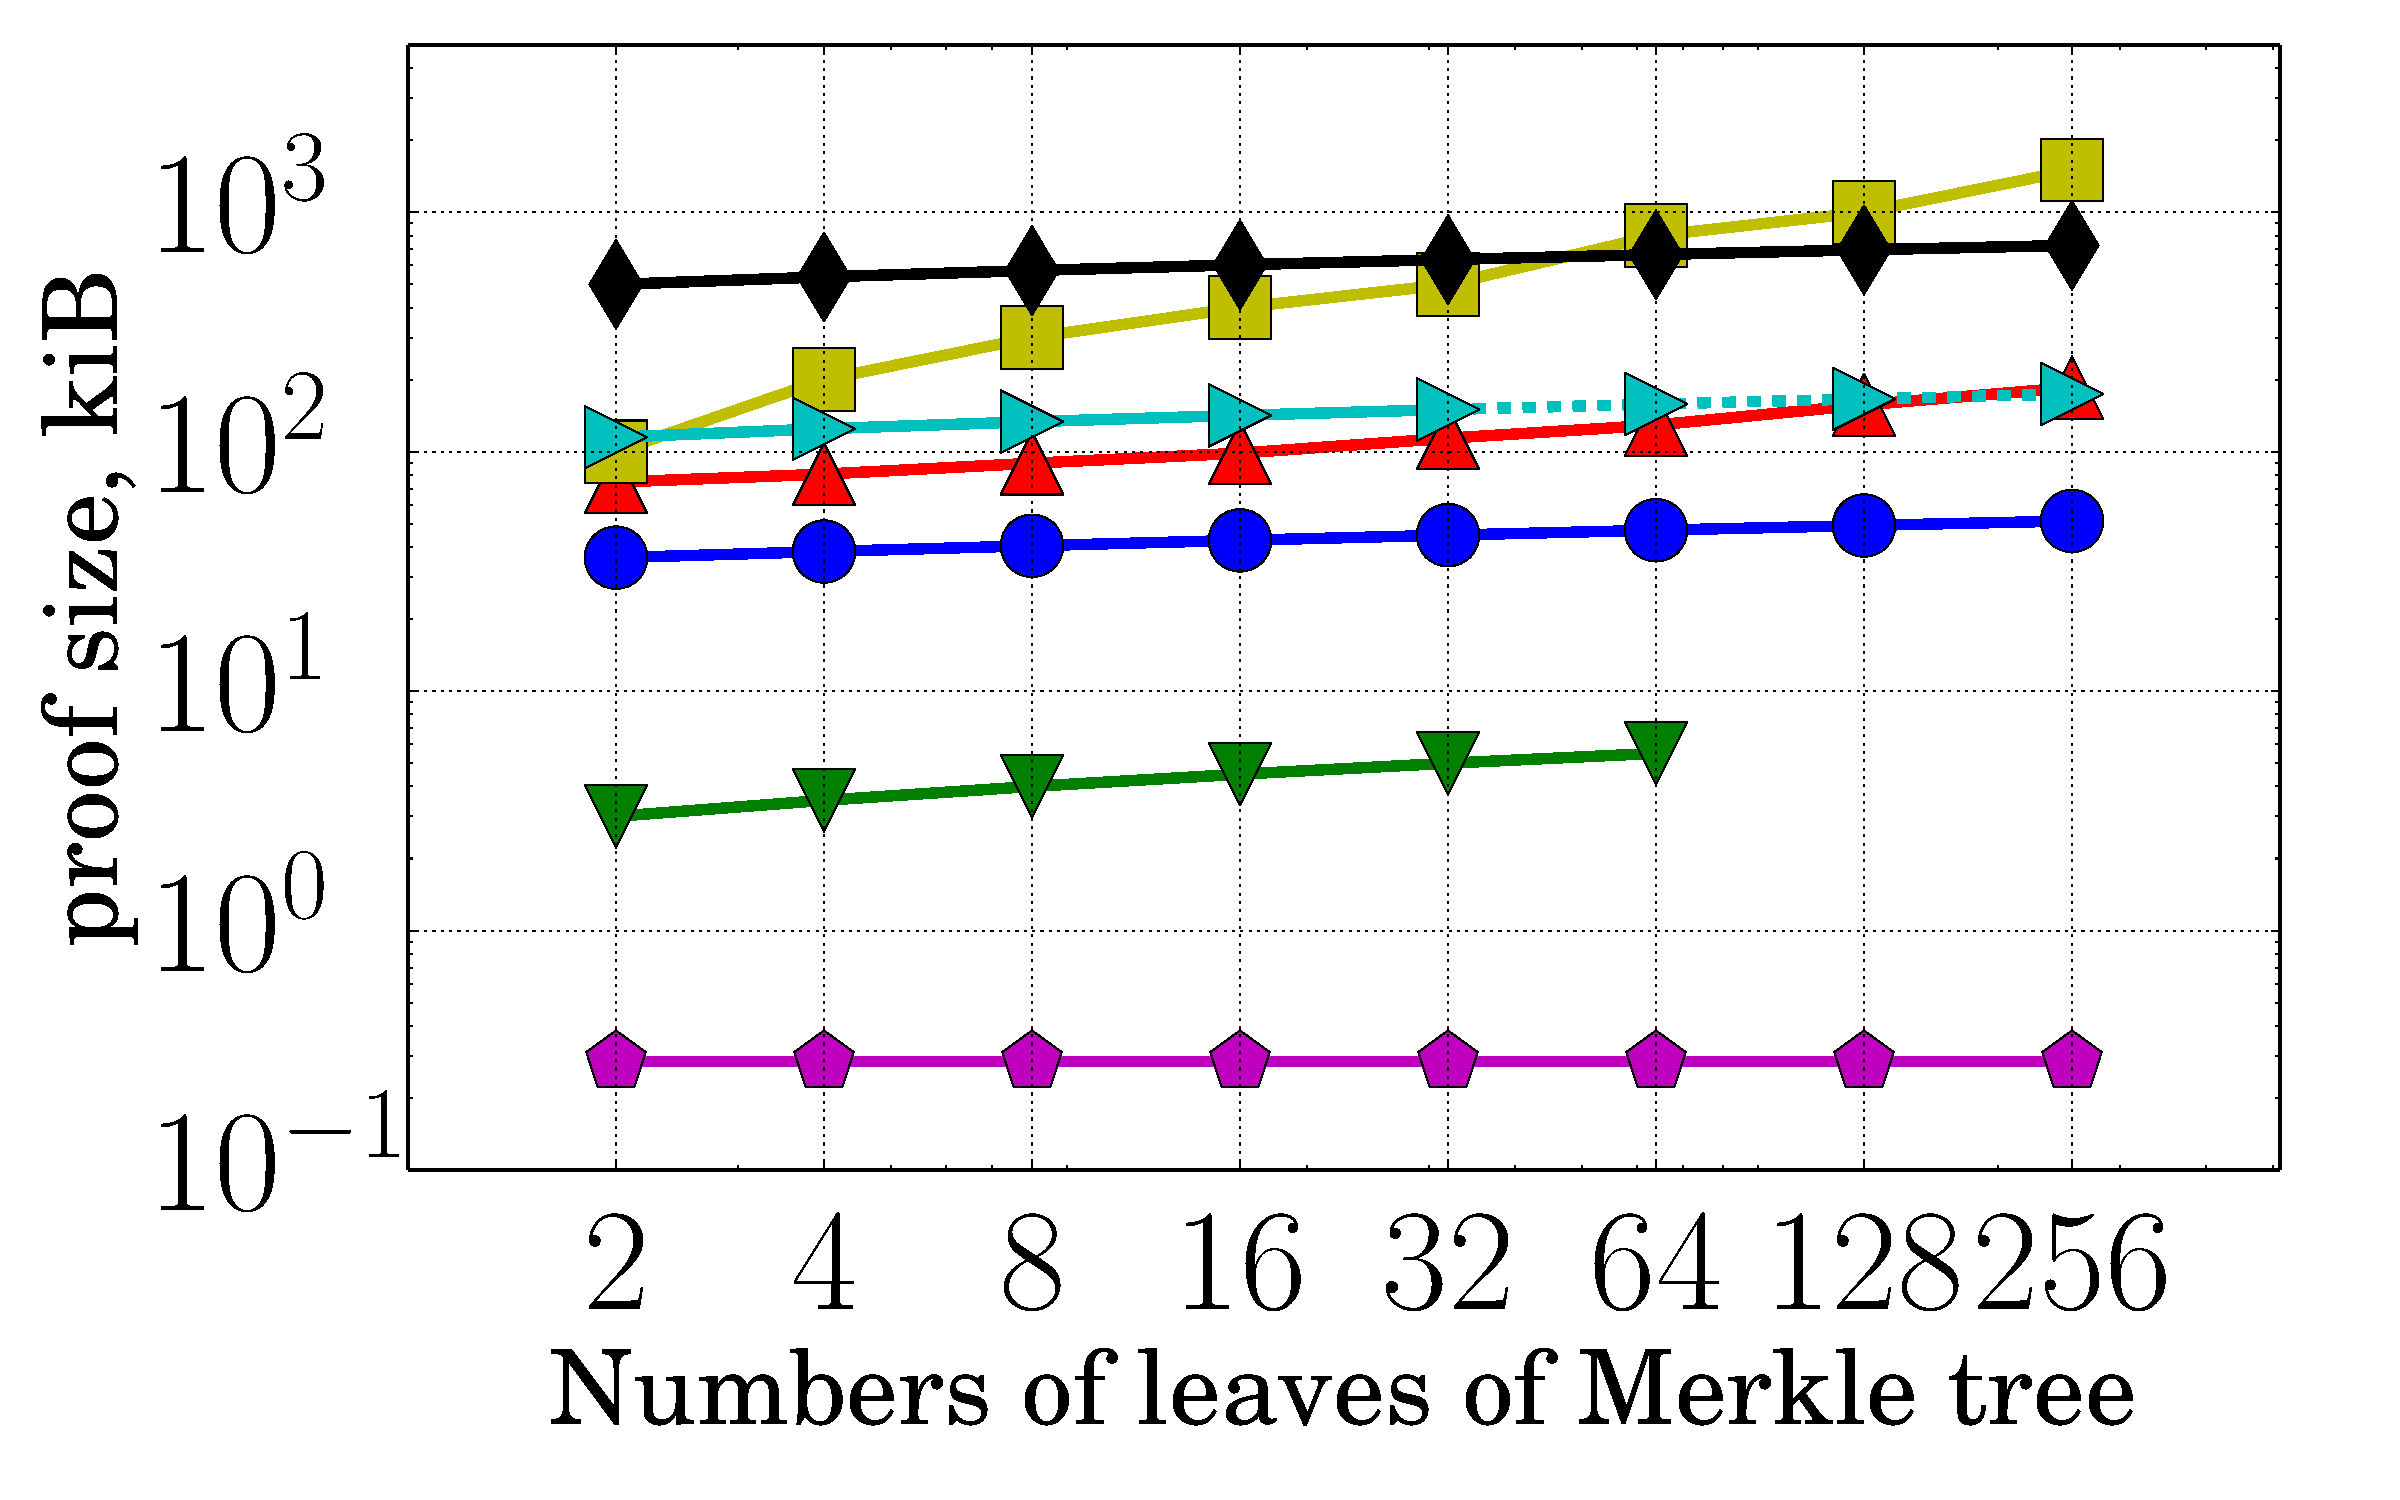
\includegraphics[width=2.1in]{fig3.pdf}
%\caption{fig2}
%\end{minipage}%
}%
\quad           
\subfigure[$\mathcal{P}$ time: 64x64 matrix multiplication]{
%\begin{minipage}[t]{0.25\linewidth}
%\centering
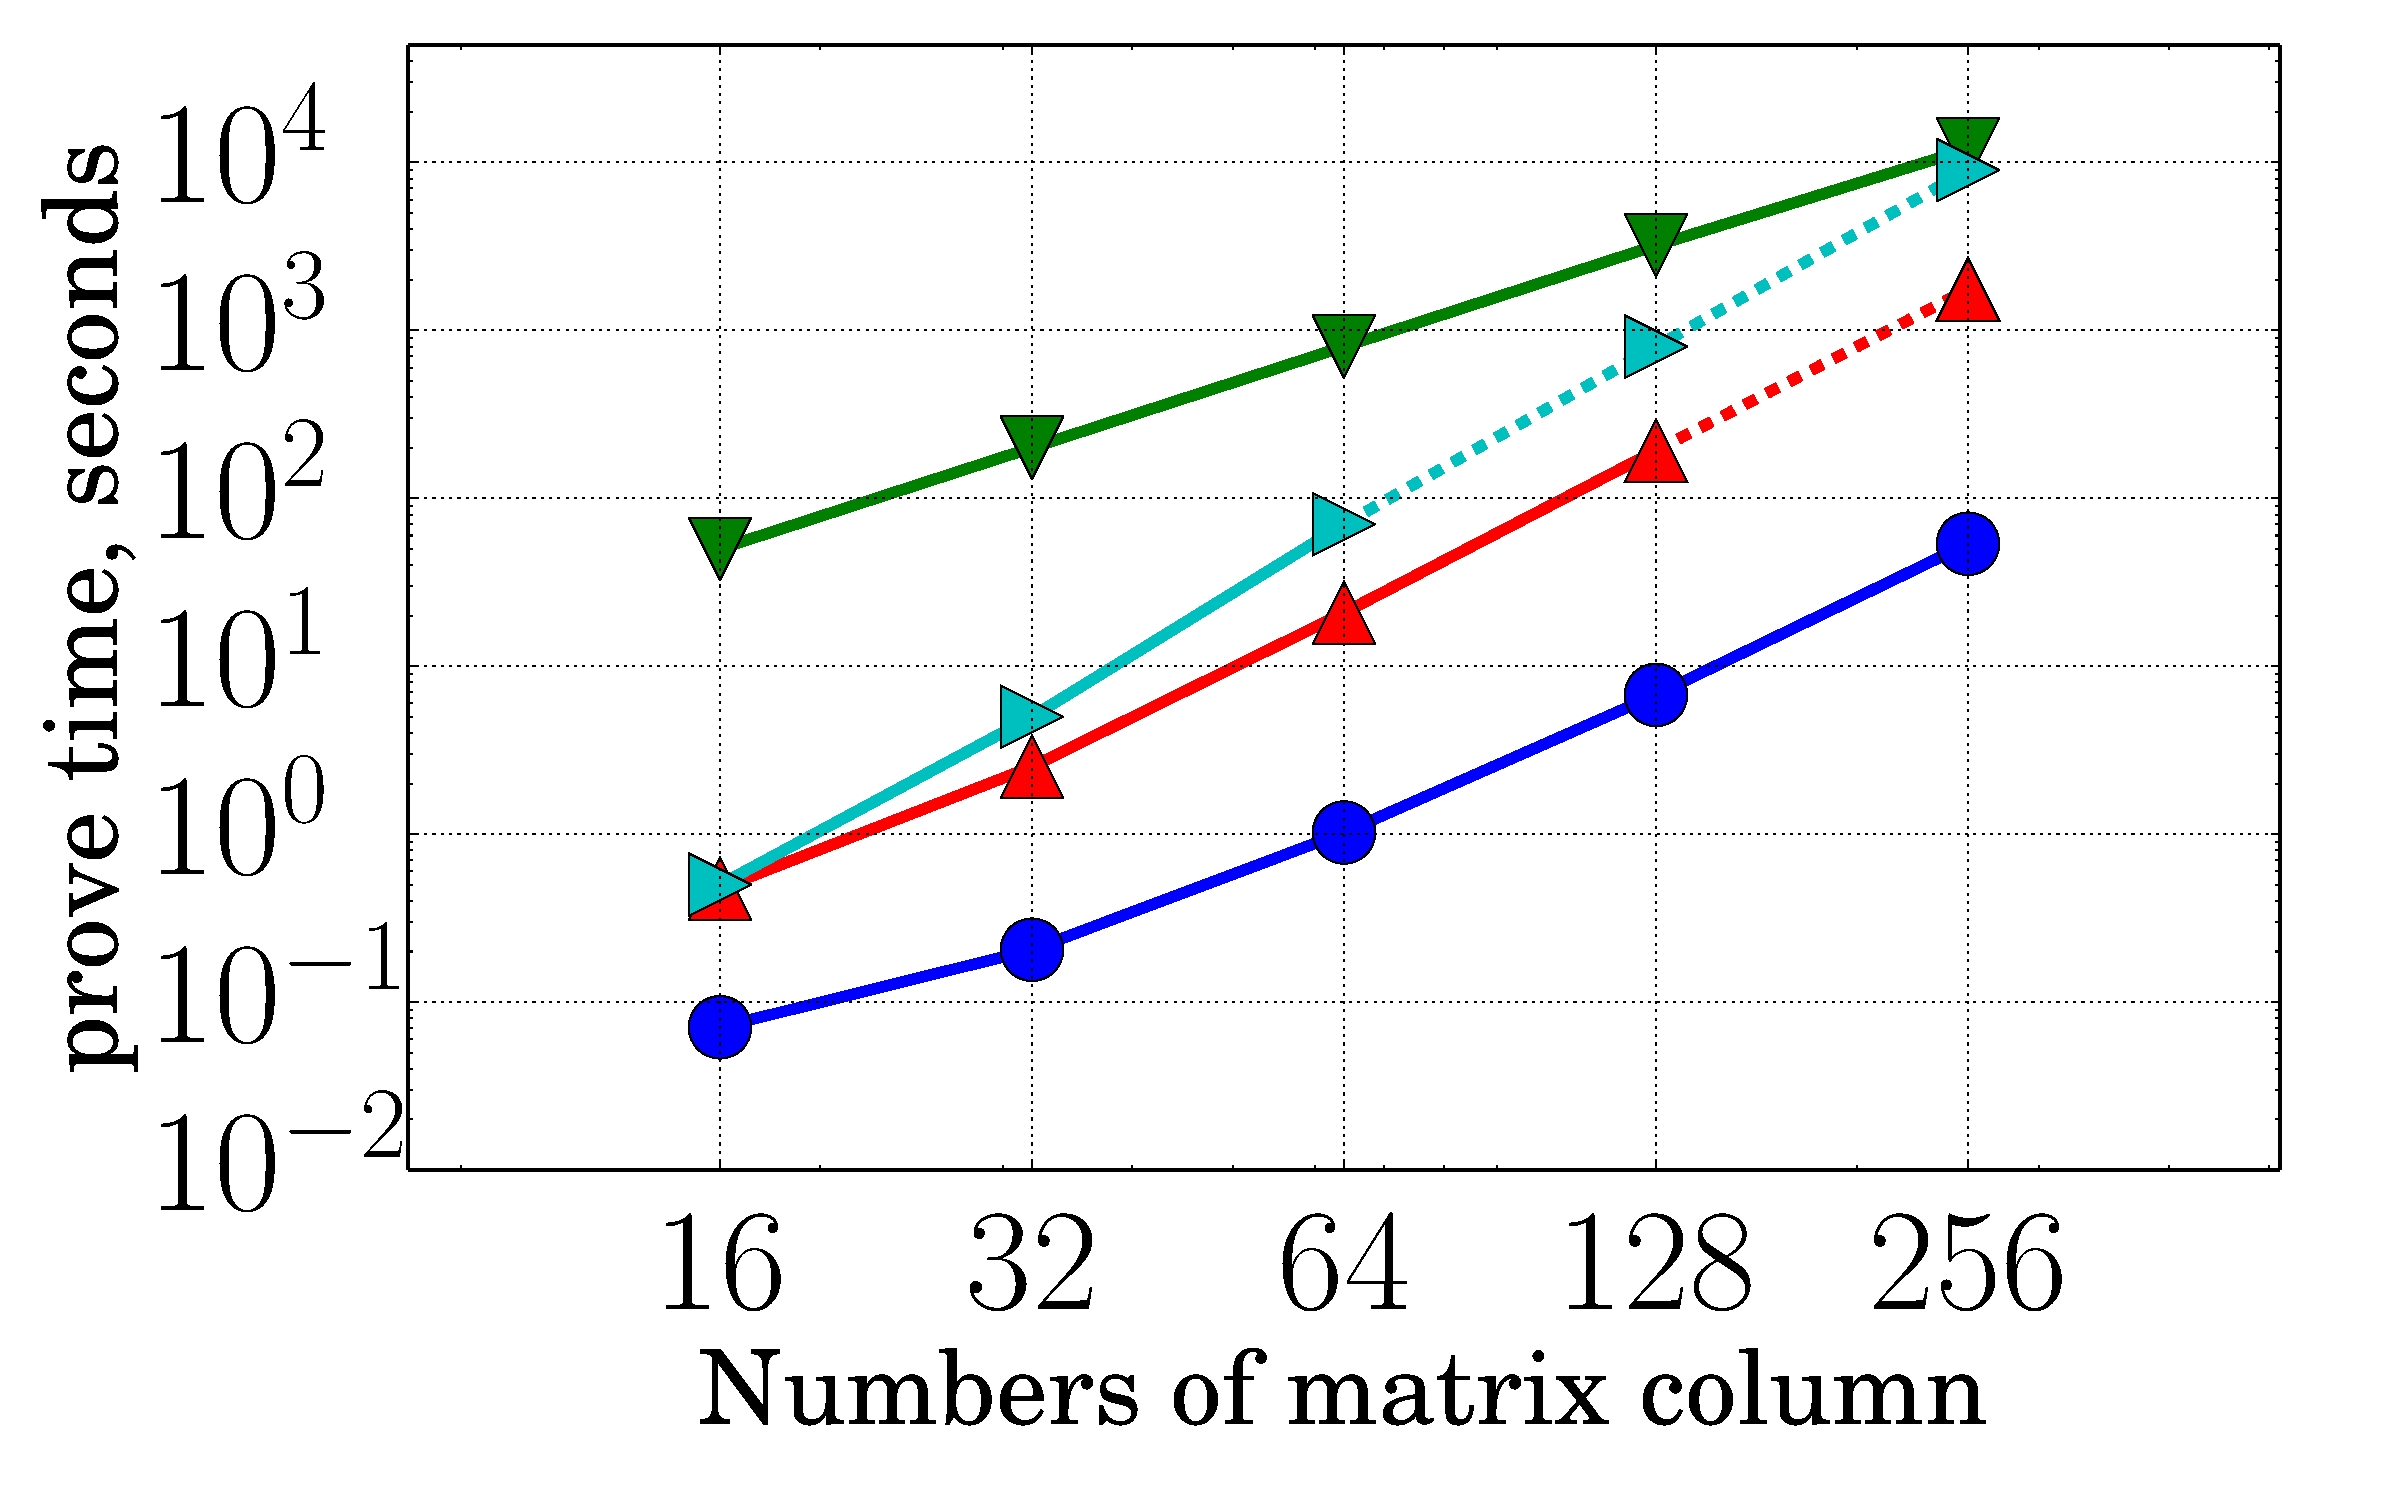
\includegraphics[width=2.1in]{fig4.pdf}
%\caption{fig2}
%\end{minipage}
}%
%\hspace{0.65in}
\subfigure[$\mathcal{P}$ time: 16x Lanczos scaling]{
%\begin{minipage}[t]{0.25\linewidth}
%\centering
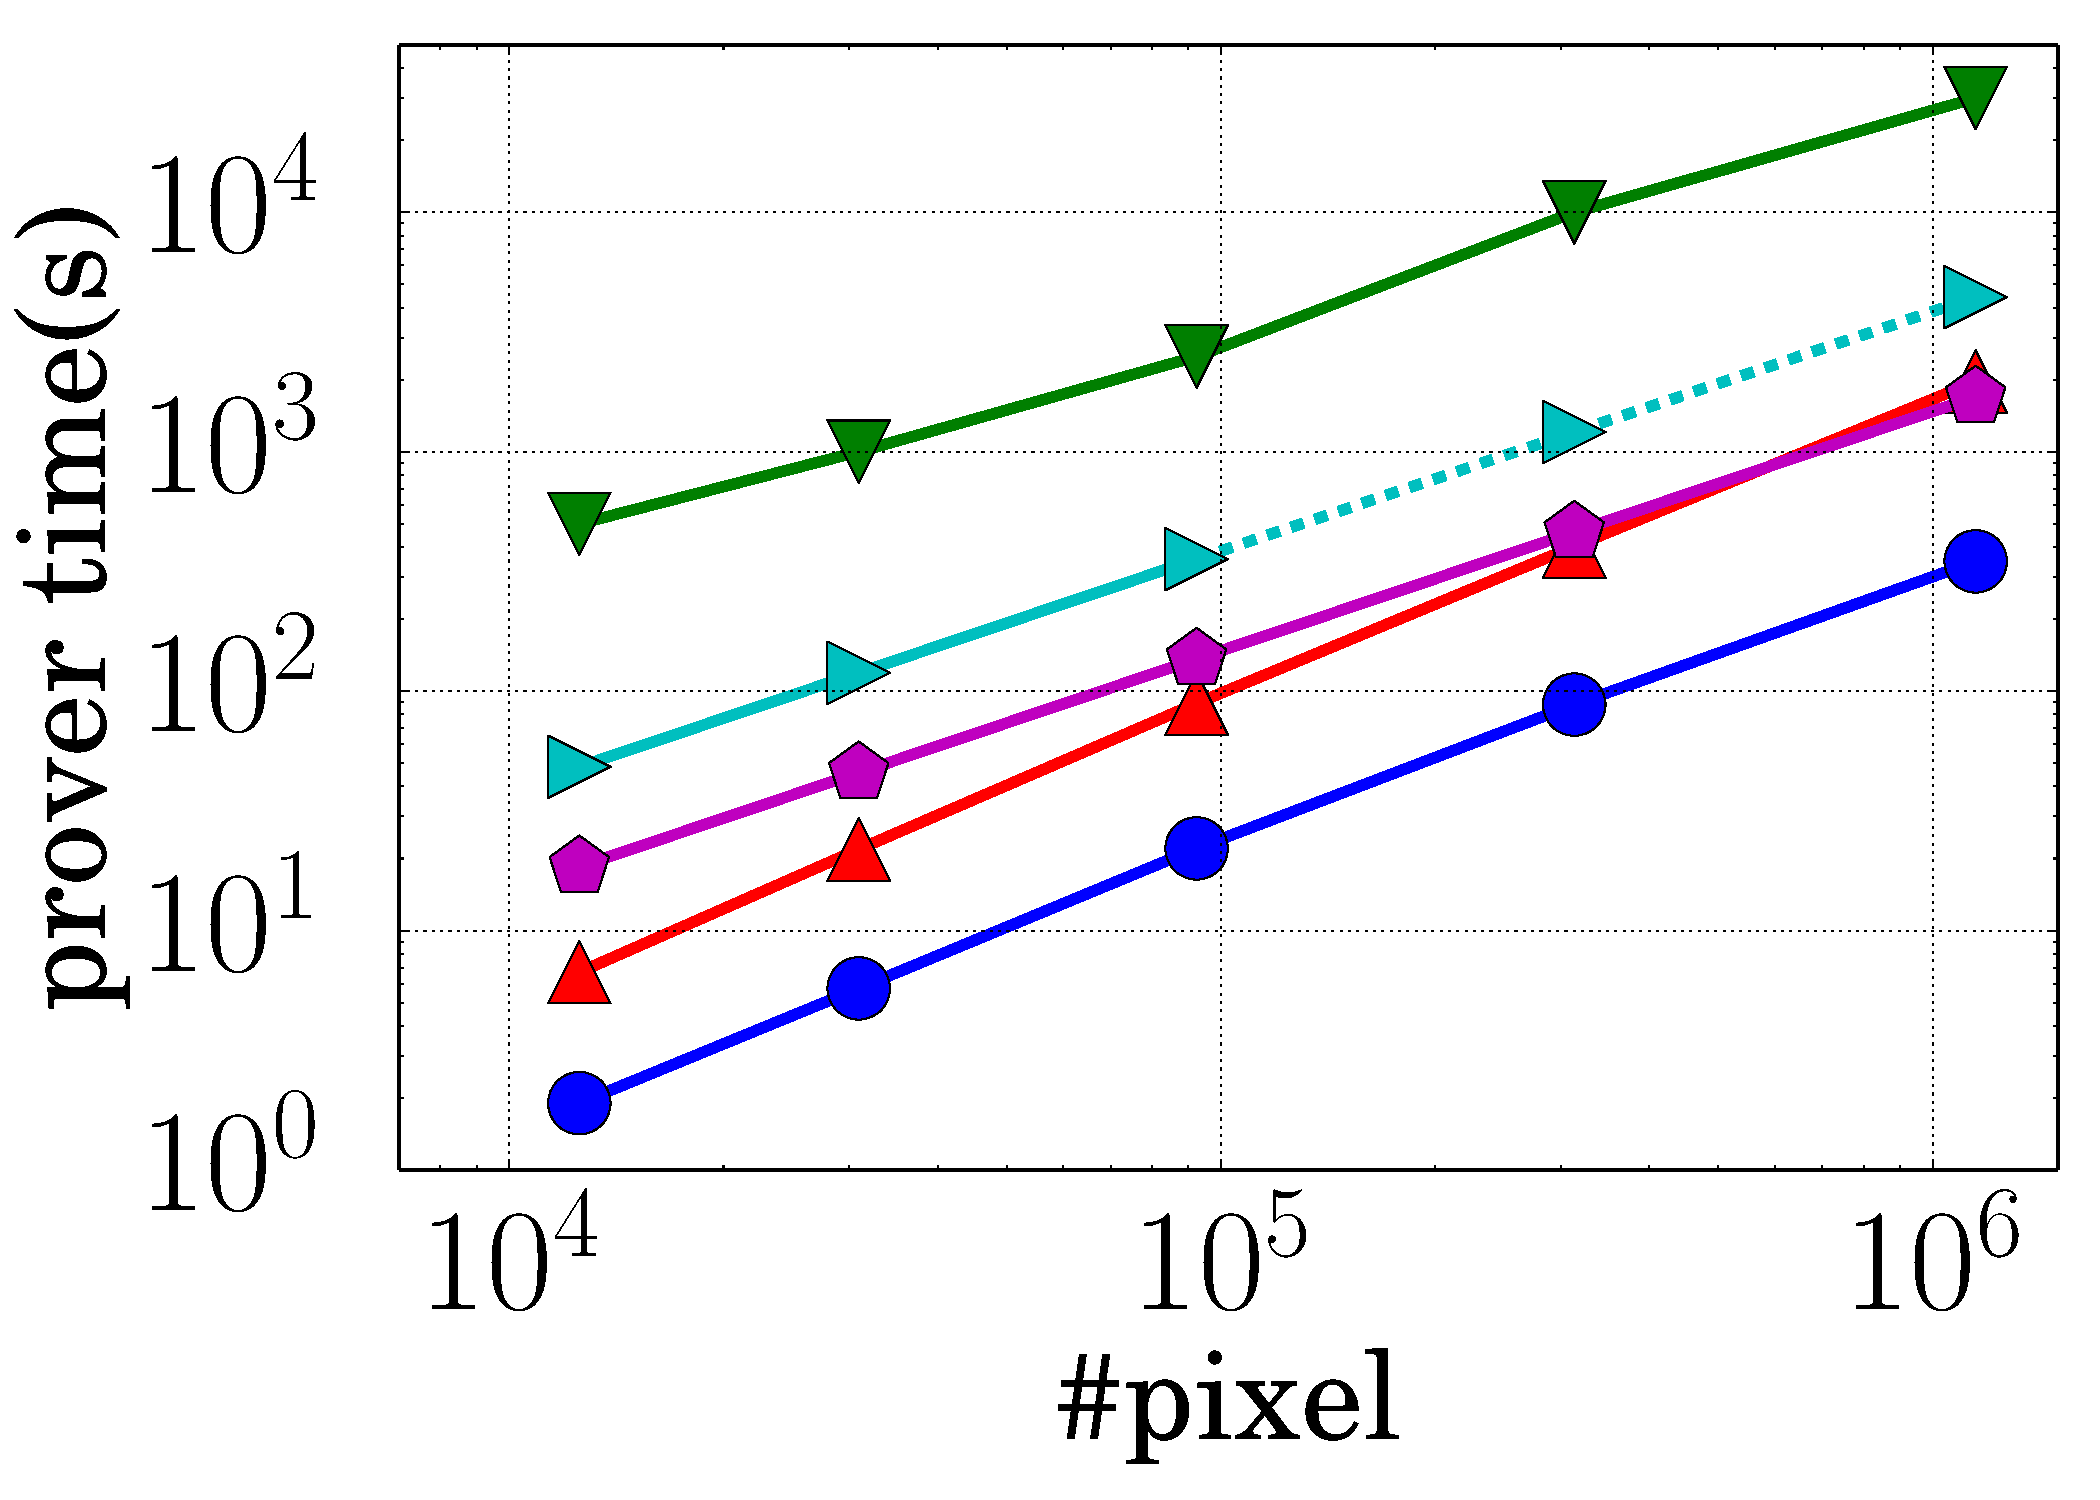
\includegraphics[width=2.1in]{fig5.pdf}
%\caption{fig2}`
%\end{minipage}
}%
%\hspace{0.65in}
\subfigure[$\mathcal{P}$ time: SHA-256 Merkle tree]{
%\begin{minipage}[t]{0.25\linewidth}
%\centering
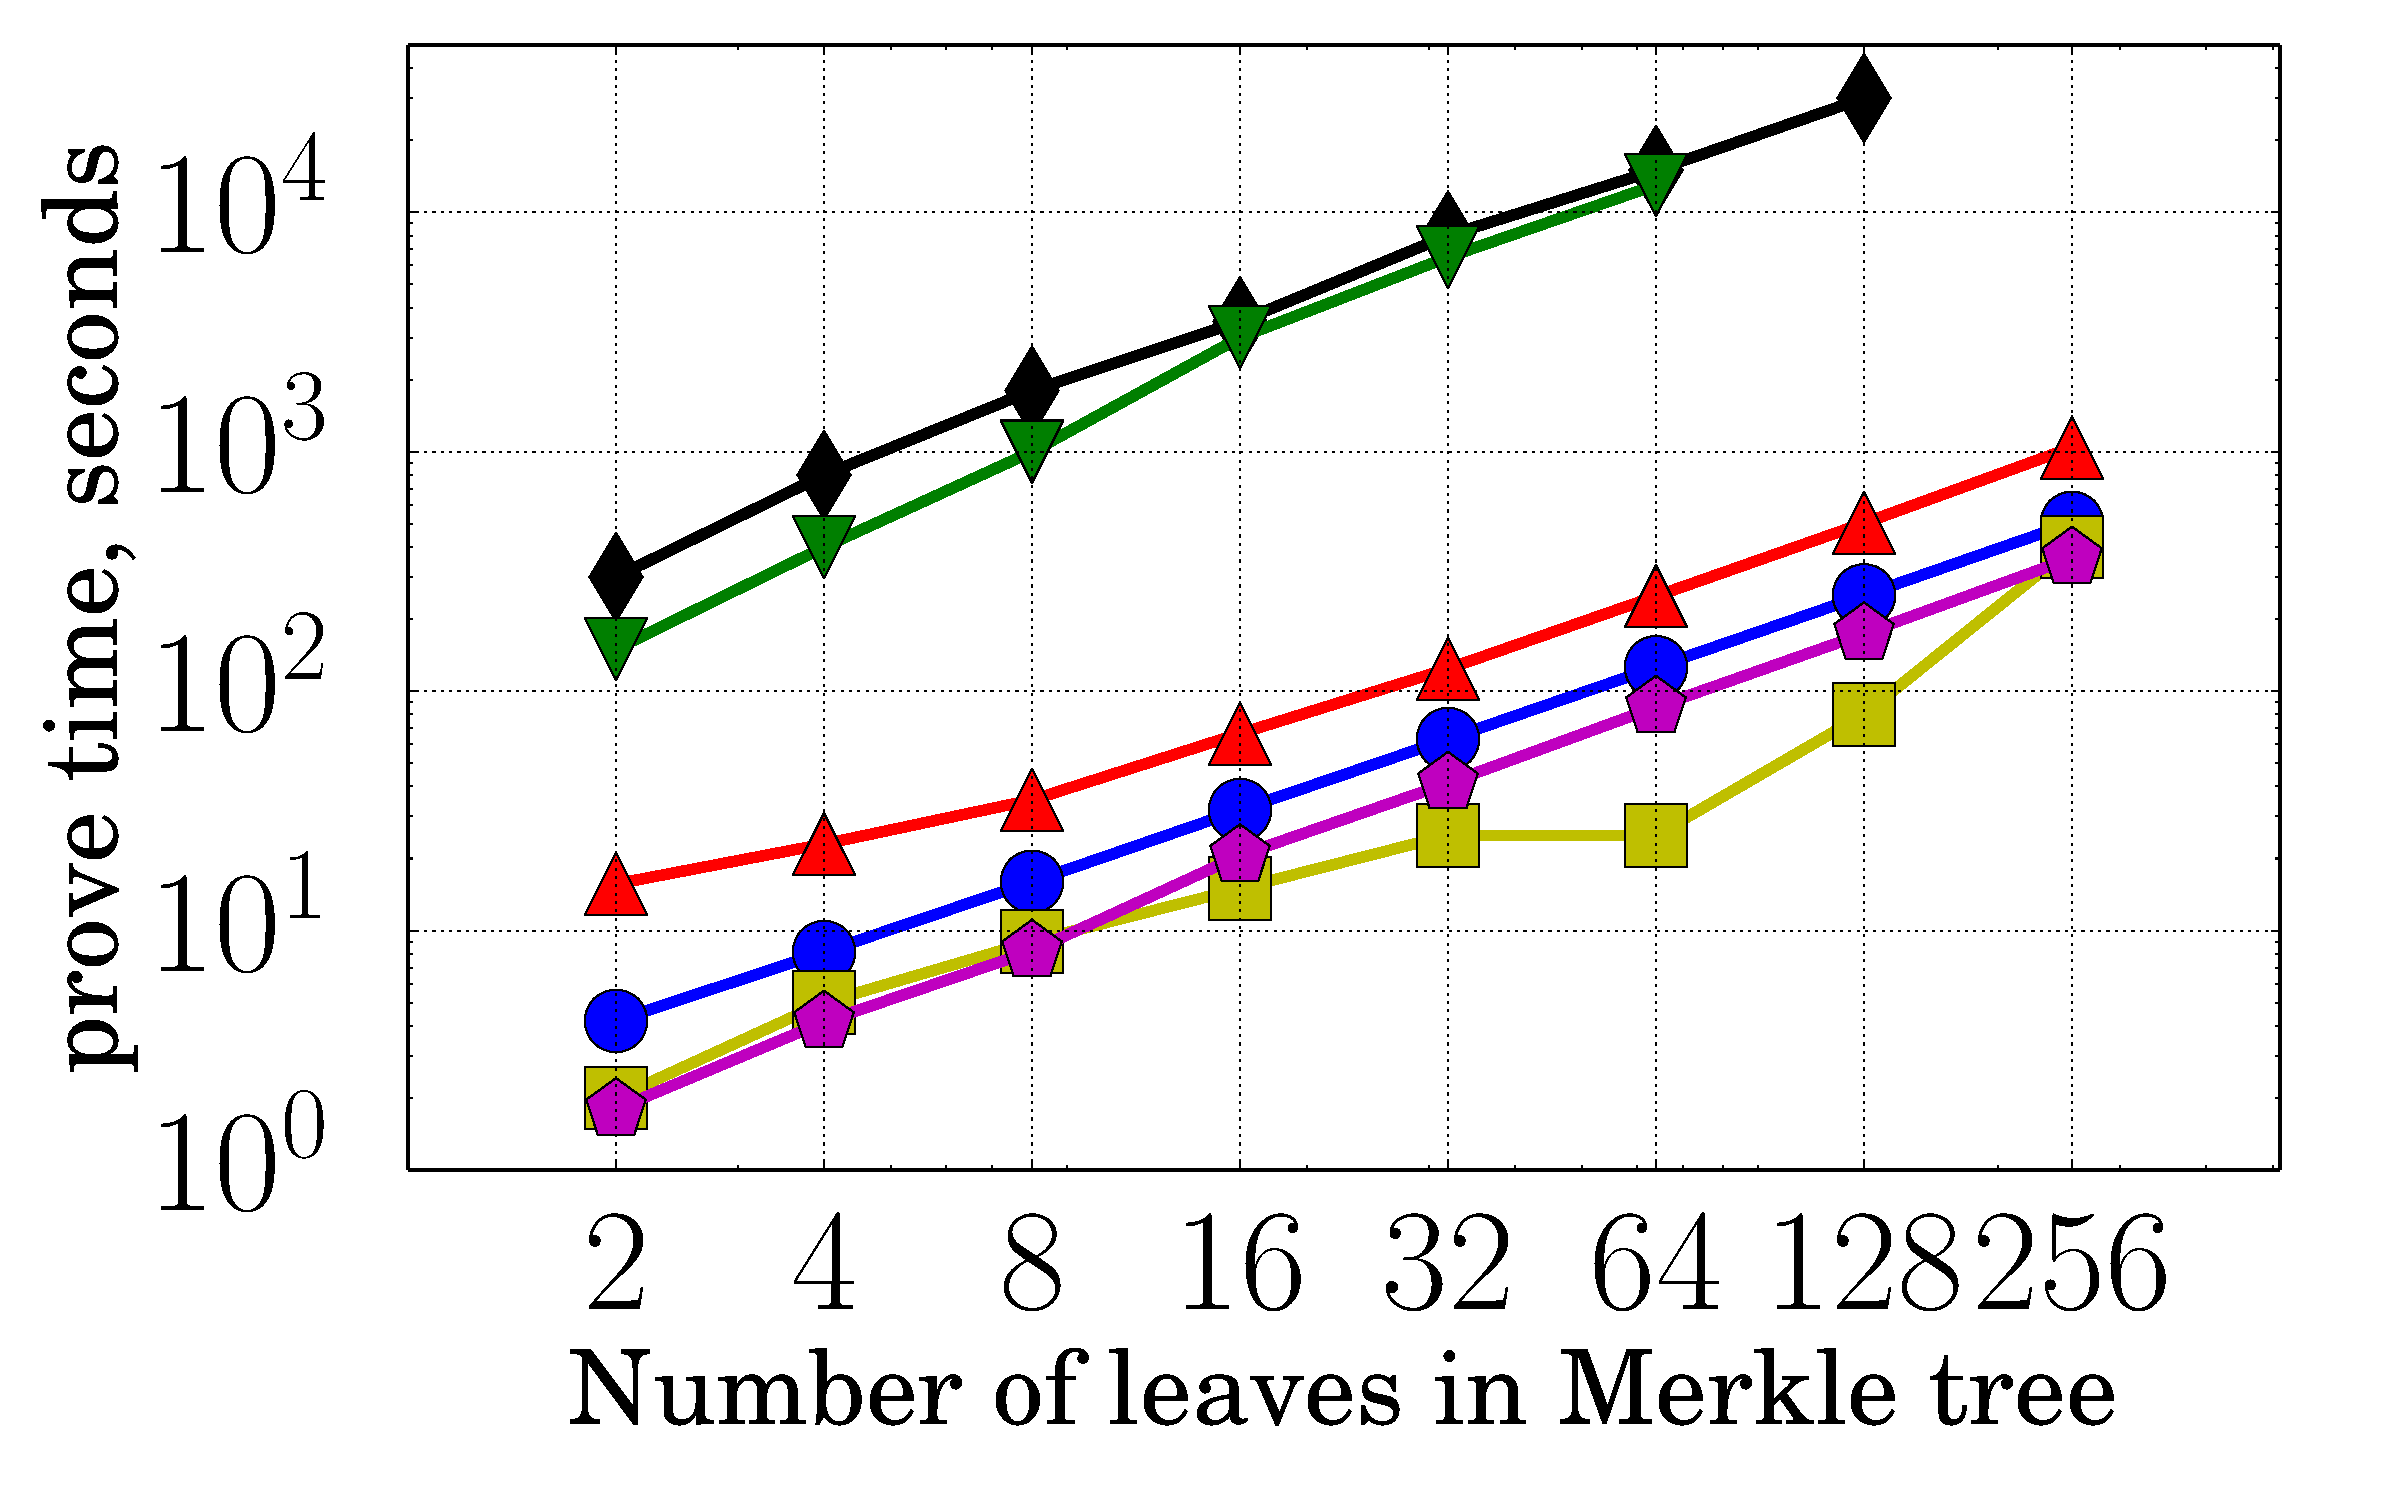
\includegraphics[width=2.1in]{fig6.pdf}
%\caption{fig2}`
%\end{minipage}
}%
\quad           
\subfigure[$\mathcal{V}$ time: 64x64 matrix multiplication]{
%\begin{minipage}[t]{0.25\linewidth}
%\centering
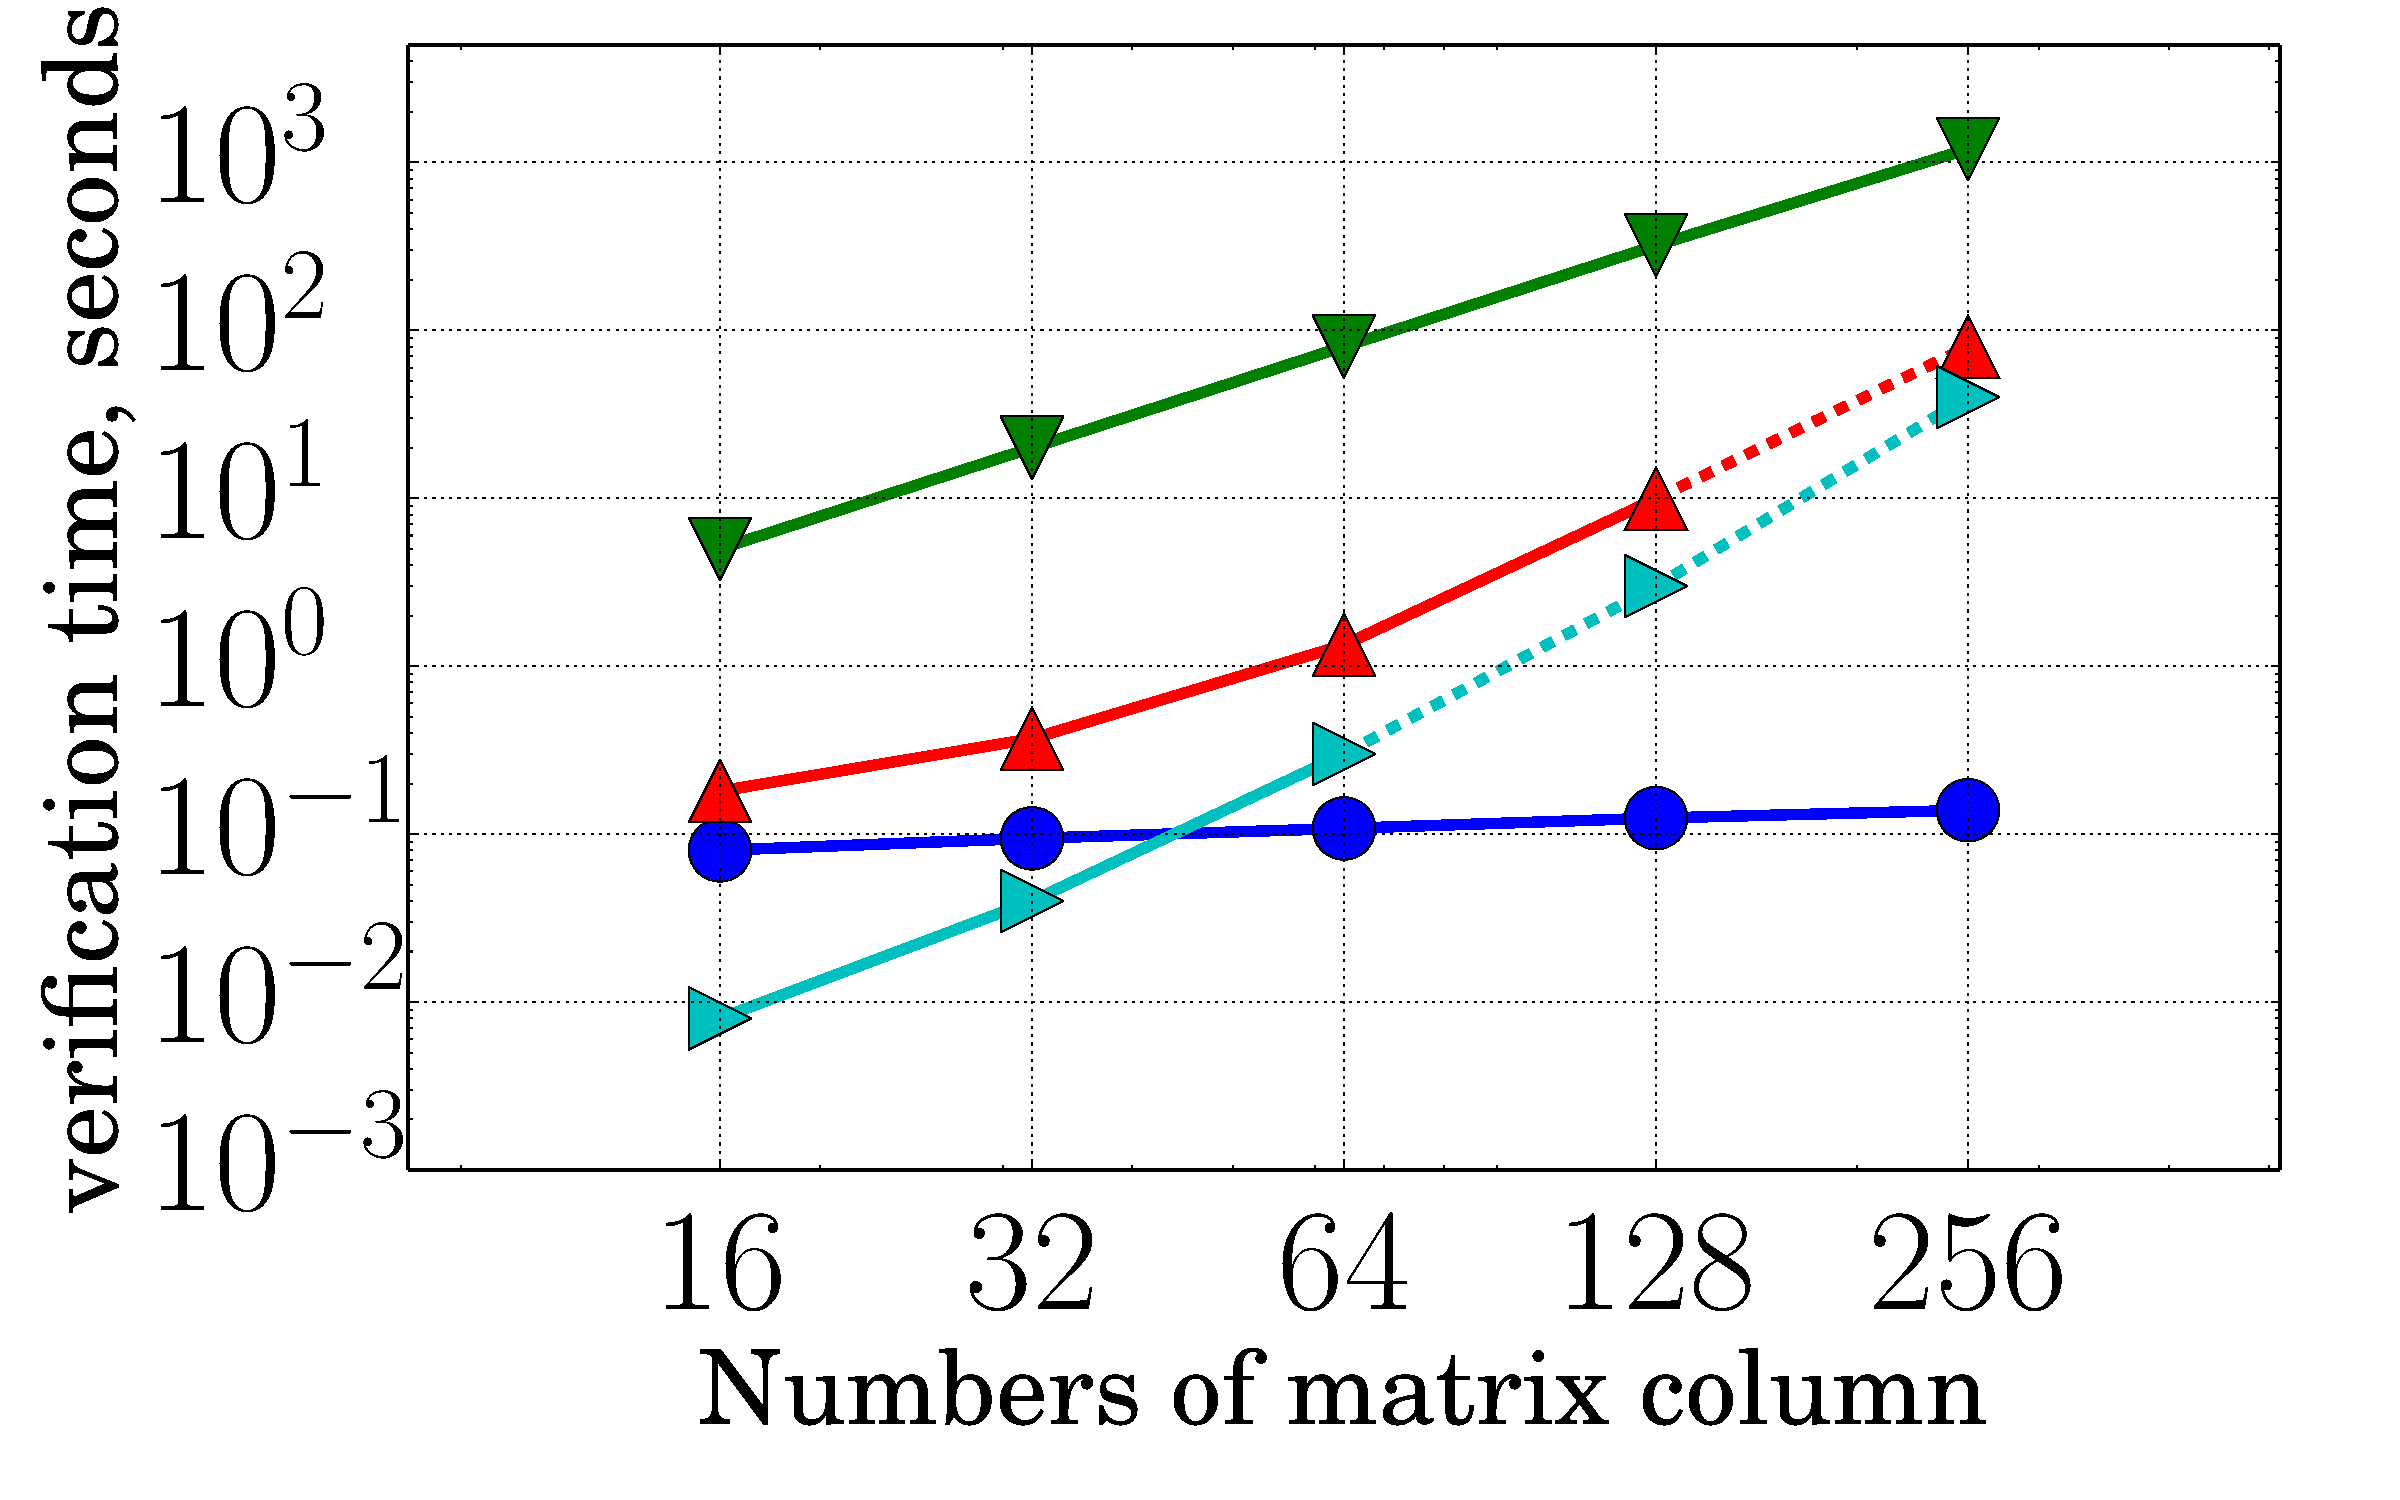
\includegraphics[width=2.1in]{fig7.pdf}
%\caption{fig2}
%\end{minipage}
}%
%\hspace{0.65in}
\subfigure[$\mathcal{V}$ time:16x Lanczos scaling]{
%\begin{minipage}[t]{0.25\linewidth}
%\centering
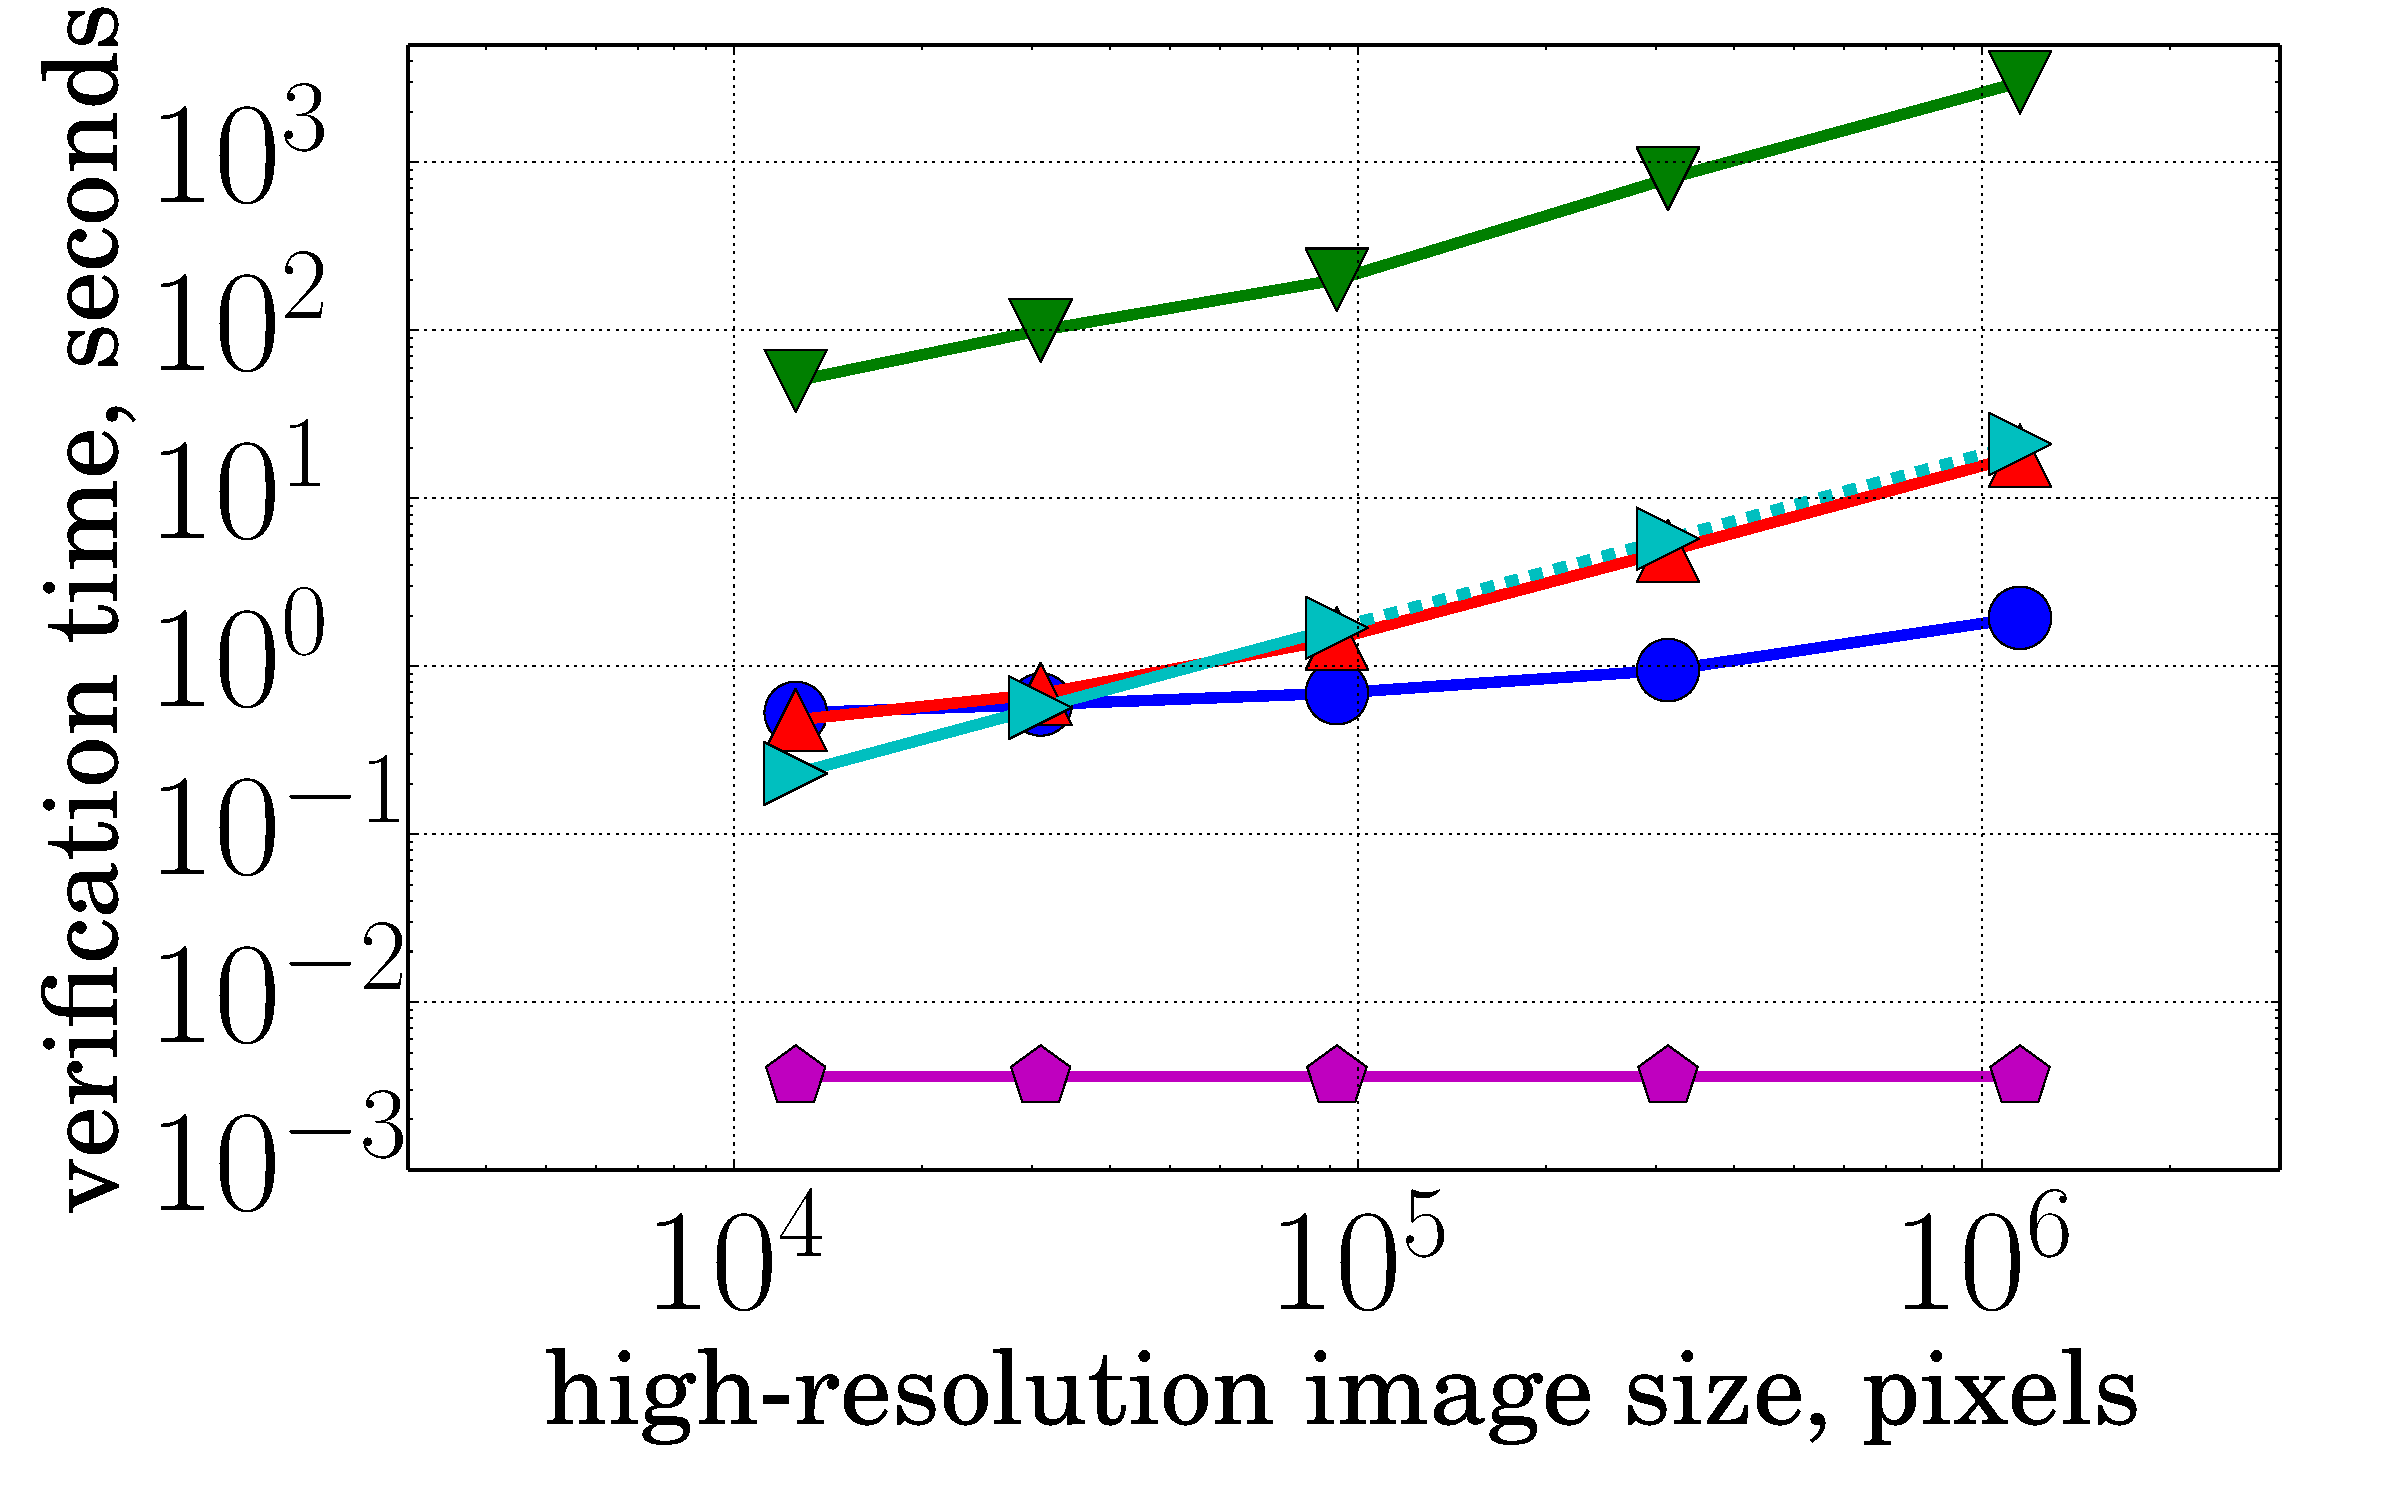
\includegraphics[width=2.1in]{fig8.pdf}
%\caption{fig2}`
%\end{minipage}
}%
%\hspace{0.65in}
\subfigure[$\mathcal{V}$ time:SHA-256 Merkle tree]{
%\begin{minipage}[t]{0.25\linewidth}
%\centering
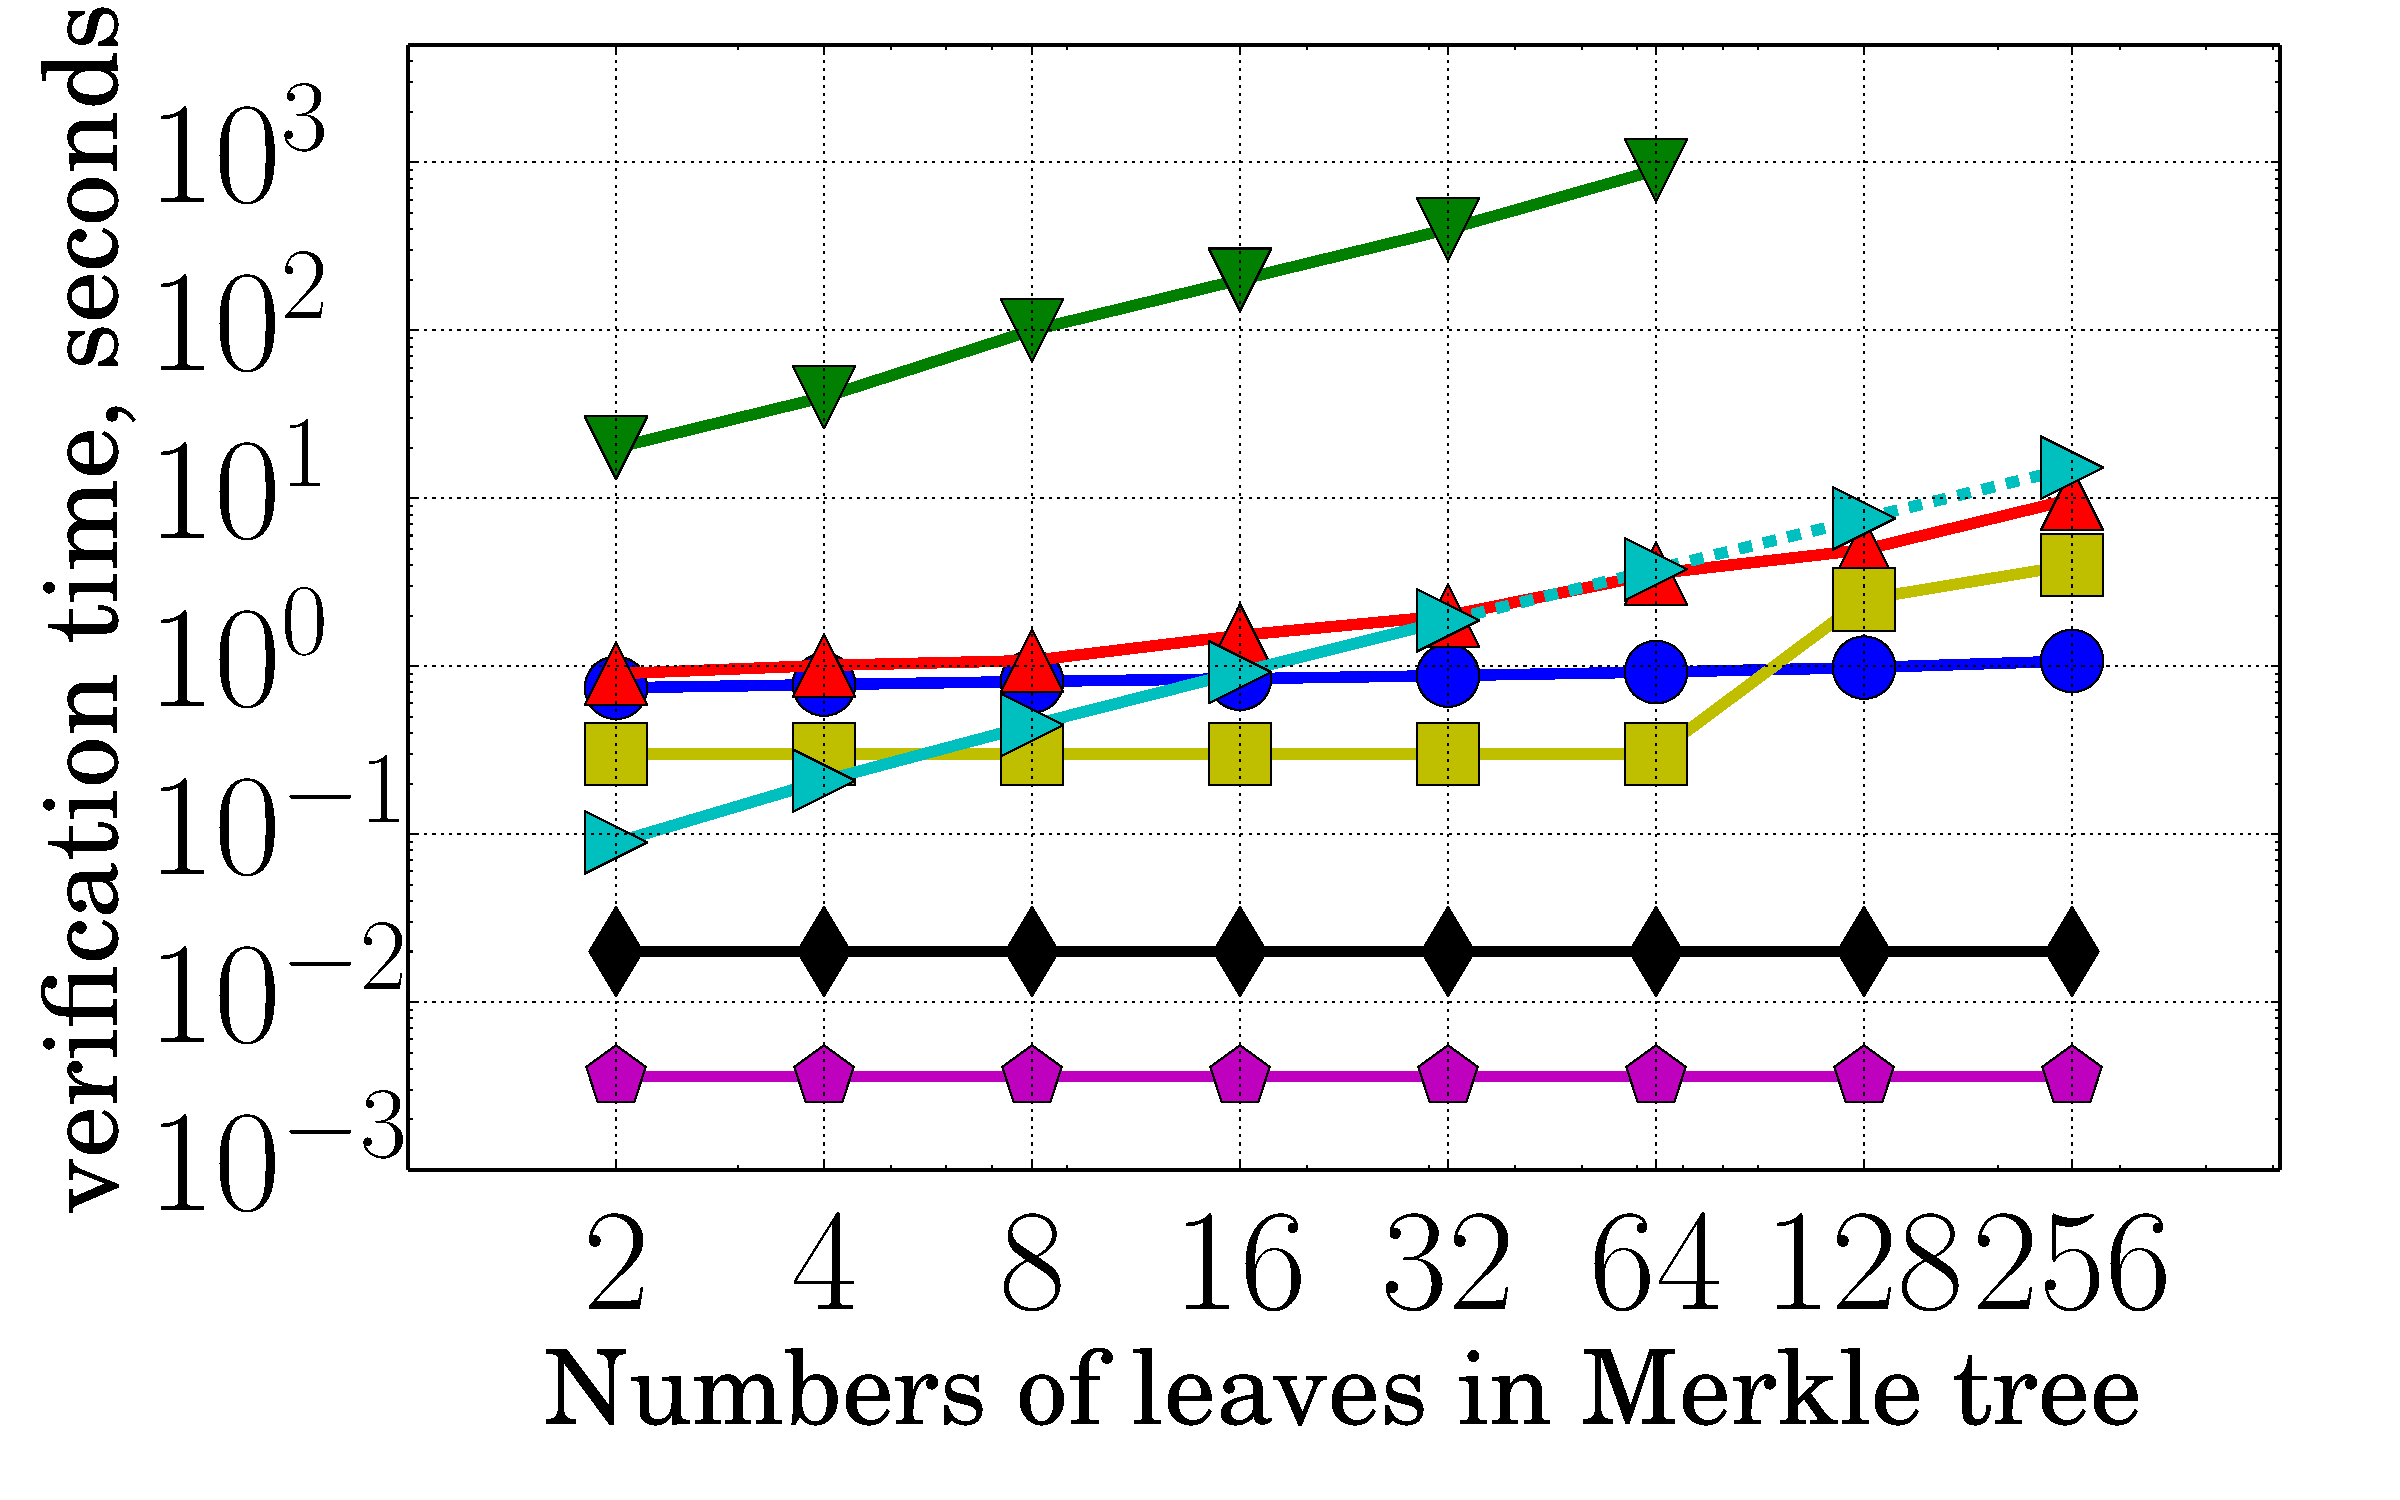
\includegraphics[width=2.1in]{fig9.pdf}
%\caption{fig2}`
%\end{minipage}
}%
%\centering
\quad
\centering

\includegraphics[width = 6.5in]{legend.pdf}
\caption{\label{ZKGKR}Comparison of the performance of \name{} versus other zero knowledge systems.}
\end{figure}

\paragraph{Experimental results.} All of experimental results are summarized in Figure \ref{ZKGKR}. We would analyse the consequences from four perspectives: prove time, verification time, proof size and memory consumption.
\begin{itemize}
	\item \textbf{prove time}: Generally, the prove time of \name{} is comparable with Ligero and much faster than any other systems. That is because Ligero is not based on the public key cryptography. For instance, for matrix multiplication, when the matrix size is 128x128, our system's prove time is roughly 5x speed up of Hyrax, 100x speed up of libSTARK and only a little slower than Ligero. For image scaling, when the number of pixels are 1072x1072, our system is...
	\item \textbf{verification time}: Generally, the verification time of \name{} is faster all other systems except libSTANK and lib SNARK. The reason is that the verifiers in libSTANK and libSNARK only have constant cost. For Merkle tree, when the leaves of Merkle tree is 256, our verification time is 3x faster than Hyrax and 2x faster than but libSTARK remains the constant. 
	\item \textbf{proof size}: For proof size, our system is smaller than other systems except for Bulletproofs since the proof size of Bulletproofs is constant while ours is logarithmic. For Merkel tree, when the number of leaves are 256, Hyrax's proof size is about 5x larger than ours while libSTARK's proof size is 10x larger than ours, but Bulletproofs' proof size remains constant.  
	\item \textbf{memory consumption}: LibSTARK, libSNARK and Bulletproofs are all high memory consumed. They run out of RAM for the medium size of the test data for matrix multiplication and Merkle tree. Our system is comparable with Hyrax and Ligero.
\end{itemize}

\subsection{Discussion}

\paragraph{Improving verification time.}

VPD for each layer

\paragraph{Removing trusted setup.}